\documentclass[a4paper,12pt]{report}

\usepackage{amsmath}
\usepackage{unicode-math}
\usepackage{polyglossia}
\usepackage{csquotes}
\setmainlanguage{russian}
\setotherlanguage{english}
\defaultfontfeatures{Ligatures={Common,TeX}}
\setmainfont{CMU Serif}
\setsansfont{CMU Sans Serif}
\setmonofont{CMU Typewriter Text}
\setmathfont{XITS Math}

\usepackage{hyperref} % for refs and URLs
\usepackage[backend=bibtex]{biblatex} % for bibliography
\usepackage{graphicx} % for images (and title page)
\usepackage{geometry} % for margins in title page
\usepackage{tabu} % for tabulars (and title page)
\usepackage{rotating} % for rotated labels in tables
\usepackage{tikz} % for TiKZ
\usepackage{dot2texi} % for inline dot graphs
\usepackage{listings} % for listings 
\usepackage{multirow} % for multirow cells in tabulars
\usepackage{afterpage} % for nice landspace floats
\usepackage{pdflscape} % for landspace orientation

\usetikzlibrary{shapes,arrows,trees}

\lstset{
language={C},
columns=fullflexible,
numbers=left,
numberstyle=\scriptsize,
captionpos=b,
extendedchars=\true,
texcl=true,
mathescape=true
}
\renewcommand{\lstlistingname}{Листинг}

\numberwithin{equation}{section}

\title{Драйвер для осциллографа Velleman PCSGU250 для ОС GNU/Linux}
\author{Амиантов Николай, ИУ7-62}
\date{\today}

\addglobalbib{summary}

\renewcommand{\thesection}{\arabic{section}}

\makeatletter
\let\thetitle\@title
\let\theauthor\@author
\let\thedate\@date
\makeatother

\begin{document}

\newgeometry{margin=1cm}
\begin{titlepage}
\begin{center}
\emph{Федеральное государственное бюджетное образовательное учреждение высшего
  профессионального образования}
\begin{tabu} to \linewidth {lX[1,c,m]}
\hline \\

\includegraphics[width=0.15\linewidth]{crest} &
\large\emph{``Московский государственный технический университет имени Н.Э.
  Баумана'' (МГТУ им. Н.Э. Баумана)} \\
\end{tabu}
\end{center}
\begin{tabu}{ll}
\large\textsc{Факультет:} & Информатика и системы управения \\
\large\textsc{Кафедра:} & Программное обеспечение ЭВМ и информационные технологии \\
\end{tabu}
\vspace{1.0cm}
\begin{center}
\huge{Расчётно-пояснительная записка} \\
\vspace{0.5cm}
\Large{по курсовой работе по системному программированию на тему:} \\
\vspace{0.3cm}
\Large{``\thetitle''}
\end{center}
\vfill
\begin{tabu} to \linewidth {Xr}
Студент \theauthor & $\underset{\text{(Подпись, дата)}}{\text{\underline{
      \makebox[5cm]{}}}}$ \\
Научный руководитель Алексеев Юрий Евтихович & $\underset{\text{(Подпись, дата)}}{\text{\underline{
      \makebox[5cm]{}}}}$ \\
\end{tabu}
\vspace{0.2cm}
\begin{center}
Москва \the\year
\end{center}
\end{titlepage}
\restoregeometry

\tableofcontents
\newpage

\section*{Введение}
Осциллограф представляет собой устройство для анализа высокочастотных цифровых
(или аналоговых) сигналов. Он позволяет демонстрировать фрагменты сигнала в
очень большом разрешении, иногда из нескольких источников одновременно, и
синхронизовать получение этих фрагментов по входящим импульсам. Он является
одним из основных инструментов для отладки и изучения электрических схем.
Существует много видов и форматов осциллографов, но в последнее время большую
популярность приобрели осциллографы, подключающийся к компьютеру, что позволяет
производить глубокий анализ полученных данных уже на ЭВМ. К сожалению, такие
осциллографы --- устройства, не соответствующие ни одному из заданных стандартом
USB классов и драйвера к ним поставляются только производителем для некоторого
набора операционных систем.

Цель работы --- разработка драйвера для USB-осциллографа c двумя каналами и
генератором сигналов Velleman PCSGU250 для операционной системы Linux. В рамках
данной работы были изучены способы написания драйверов для ядра Linux, работа с
подсистемами ядра и способы передачи данных между режимами пользователя и
ядра.

\newpage
\section{Аналитический раздел}
\subsection{Задача}
В соответствии с задачей необходимо разработать драйвер для осциллографа
Velleman PCSGU250 с подключением по USB, который обеспечивает работу устройства
и при этом не влияет на общую работу системы.

\subsection{USB-шина}
\subsubsection{Анализ шины}
USB-шина является последовательной шиной для подключения практически любых
устройств к компьютеру. В настоящий момент это крайне распостранённая
технология, позволяющая подключать целый спектр различных устройств ``на
горячую'' (hotplug) к компьютеру. Благодаря простоте стандарта и введённыму в
него понятию ``класса устройства'' многие устройства не требуют драйвера для
работы и запускаются ``из коробки'', так как соответствуют стандартам USB на
определённый класс устройств. Технология USB позволила отказаться от множества
старых интерфейсов (PS/2, COM, LPT) и подключать практически любые устройства,
используя одну шину.

\subsubsection{Топология шины}
USB-шина построена по ассиметричной топологии, в которой выделяется ``хост'',
множество USB-портов и устройства, подключённые по топологии ``многоуровневая
звезда''. На каждом уровне может быть один или больше USB-разветвлителей, дающих
возможность создавать степень ветвления шины до пятого уровня включительно.
Пример такого дерева даётся на рисунке~\ref{sampleusbtree}. Включая хабы, к
хосту может быть подключено до 127 устройств.~\cite{usb20} Такая архитектура
проста в исполнении, позволяет подключать множество устройств одновременно и
удобна для пользователя. В шине между хостом и устройствами создаются соединения
``точка-точка''. У каждого устройства может существовать одна или больше точек
входа (endpoints), каждая из которых является однонаправленным каналом передачи
данных определённого типа. Устройство само по себе не может посылать данные
хосту, контроллер должен опрашивать устройства на шине на наличие новых
данных. Это решает проблемы с обеспечением свободной шины для передачи данных и
в целом сильно упрощает архитектуру.

\begin{figure}[h!]
\centering
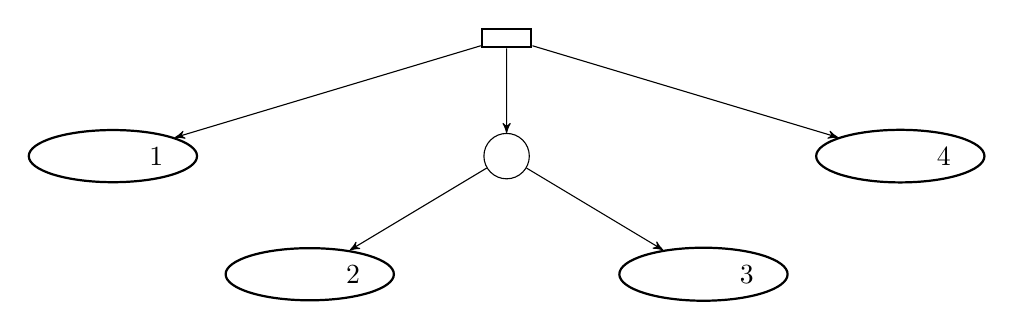
\begin{tikzpicture}[->,grow=down,>=stealth',level/.style={sibling distance = 5cm,
  level distance = 1.5cm},
usbhost/.style = {draw, rectangle, thick, black, font=\sffamily\bfseries},
usbdevice/.style = {draw, ellipse, thick, black, fill=none},
usbhub/.style = {draw, circle, black}
]
\node [usbhost] {Хост}
  child{ node [usbdevice] {Устройство 1} }
  child{ node [usbhub] {Хаб}
     child{ node [usbdevice] {Устройство 2} }
     child{ node [usbdevice] {Устройство 3} }
  }
  child{ node [usbdevice] {Устройство 4} }
;
\end{tikzpicture}
\caption{Пример USB-дерева}
\label{sampleusbtree}
\end{figure}

\subsubsection{Классы устройств}
Устройства объединяются в классы по функциональности. Если устройство
соответствует какому-либо классу, то написание для него особых драйверов
необязательно, и оно может работать ``из коробки'' в любой операционной
системе. Устройство может также не принадлежать ни к одному из существующих
классов --- в частности, рассматриваемый осциллограф является именно таким
устройством. Класс представляет собой стандарт, описывающий поведение
устройства, его функциональность и протокол общения с ним, создавая возможность
работать с любым устройствам класса на уровне хотя бы базовой функциональности
без дополнительных драйверов. Поддерживается также дополнительные, не
предусмотренные стандартом расширения функциональности, так что устройство может
одновременно соответствовать некоторому классу и предоставлять дополнительные
возможности, которые уже будут требовать дополнительных драйверов операционной
системы.

\subsubsection{Пример инициализации устройства}
Несколько конечных точек объединяются в ``интерфейс'', который принадлежит к
определённому классу. Во время подключения USB-контроллер хоста сначала получает
данные о:
\begin{itemize}
\item идентификаторе производителя;
\item идентификаторе модели устройства;
\item одной или нескольких виртуальных устройств опредённого класса;
\item одной или нескольких конечных точек для каждого устройства;
\end{itemize}
Затем он сообщает о новом устройстве операционной системе. В её задачу входит
определение необходимых драйверов для устройства на основе этих данных, их
загрузка и запуск.

\subsubsection{Передача данных}
Стандарт USB предусматривает несколько типов передаваемых данных. Каждая
конечная точка задаётся (кроме её номера) её направлением и типом передачи
данных. В стандарте существуют следующие типы~\cite{corbet2009linux}:
\begin{itemize}
\item CONTROL (управляющая) \\
Обычно используется для настройки устройства, получения информации из
устройства. Пакеты этого типа обычно небольшие, и все USB-устройства имеют хотя
бы одну управляющую конечную точку, называемую ``endpoint0'', которая
используется операционной системой для настройки устройства во время
подключения. Стандартом USB гарантированно, что передачи этого типа всегда
смогут дойти до устройства в определённый срок, для чего резервируется часть
пропускной способности канала.
\item INTERRUPT (прерывающая) \\
Прерывающие конечные точки передают небольшое количество данных за фиксированное
время каждый раз как хост запрашивает данные у устройства. Эти конечные точки
--- основной метод передачи данных для USB-клавиатур и мышей. Они также
используются как основной канал для настройки устройства, но обычно не
используются для передачи больших объёмов данных. Стандартом также
гарантированно, что передачи этого типа дойдут до хоста.
\item BULK (поточная) \\
Поточные конечные точки используются для передачи больших объёмов данных
(обычно гораздо больших, нежели прерывающие). Они используются для устройств
которым необходимо передавать большие объёмы данных без потерь. Стандартом не
гарантируется, что передачи по конечной точке этого типа дойдут за определённое
время. Если на шине в настоящий момент недостаёт пропускной способности чтобы
отправить целиком BULK-пакет, он разбивается на несколько передач. Эти конечные
точки используются в принтерах, дисковых и сетевых устройствах.
\item ISOCHRONOUS (изохронные) \\
Изохронные конечные точки также используются для передачи больших обхёмов
данных, однако не гарантируется что данные будут доставлены. Такие конечные
точки используются в устройствах которые предполагают частичную потерю данных,
но требуют постоянного большого потока данных через шину. Примером являются
аудио- и видеоустройства.
\end{itemize}
Для каждой конечной точки также задаётся максимальный размер пакета. Возможные
размеры пакетов прописаны в стандарте USB и не подлежат изменению; производитель
должен выбирать возможные максимальные размеры пакета из таблицы, заданной в
стандарте.~\cite{wiki:usb}

\subsubsection{Характеристики подключения устройства}
В данном осциллографе Velleman PCSGU250 для подключения по USB используется
контроллер USB 2.0 и один интерфейс с неопределённым классом устройства
(т.е. устройство требует особого драйвера) и двумя конечными точками для
дуплексного соединения типа INTERRUPT. По этим двум конечным точкам передаются
как управляющие последовательности, так и данные по определённому протоколу.

\subsection{Анализ характеристик осциллографа}
\subsubsection{Общее описание}
Осциллограф --- устройство, которое состоит из входного каскада, управляющей
логики и устройства вывода. Устройством вывода может быть как электронно-лучевая
трубка (в случае старых аналоговых осциллографов), так и другие устройства. В
нашем случае устройством вывода служит встроенный USB-контроллер, который
позволяет подключать осциллограф как slave-устройство к USB-шине, так что данный
осциллограф не является автономный. Входной каскад в осциллографе --- его
основная часть, и от его характеристик зависит, насколько точный и разрешающий
данный осциллограф. Входных каскадов может быть несколько, по количеству каналов
в осциллографе. Некоторые осциллографы также могут быть совмещены с генератором
сигналов, мультиметром (измерителем напряжения, силы тока и прочих характеристик
электрической цепи) и прочими полезными дополнительными
устройствами.~\cite{лозицкий1976электрорадио}.
% MORESHIT: Про аналоговые осциллографы и типы устройств вывода
\subsubsection{Характеристики входных каскадов}
Входные каскады различаются по нескольких характеристикам, отражающим их
качество и возможности:
\begin{itemize}
\item Разрешающая способность (максимальная частота измерения) \\
Один из важнейших параметров, определяет, насколько высокочастотный сигнал можно
просматривать и измерять с помощью устройства. Современные оциллографы способны
измерять гигагерцовые сигналы. Для измерения и просмотра более высокочастотных
сигналов применяются электронно-оптические камеры.~\cite{wiki:oscilloscope}
\item Импеданс (величина потери переменного сигнала) \label{impedance} \\
Импеданс --- это аналог сопрпотивления для контуров, на вход которых поступают
переменные сигналы. Он позволяет учитывать и амплитудные, и фазовые
характеристики сигналов и систем.~\cite{фейнман1977фейнмановские}
Импедансом $\hat{z}(j \omega)$ называется отношение комплексной амплитуды
напряжения гармонического сигнала, прикладываемого к двухполосному контуру, к
комплексной амплитуде тока, протекающего через контур. Комплексной амплитудой
называется коплексная величина, у которой модуль --- это амплитуда величины, а
аргумент --- начальная фаза. По определению:
\begin{equation}
\hat{z}(j ]omega) = \frac{\hat{u}(j \omega, t)}{\hat{i}(j \omega, t)} =
\frac{U{\omega} e^{j(\omega t + \phi_u(\omega))}}{I(\omega) e^{j(\omega t +
    \phi_i(\omega))}}
\end{equation}
Импеданс не должен зависеть от времени; если время $t$ в выражении для импеданса
не сокращается, значит, для данного двухполосника понятие импеданса
неприменимо. Соответственно:
\begin{equation}
\frac{U{\omega} e^{j(\omega t + \phi_u(\omega))}}{I(\omega) e^{j(\omega t +
    \phi_i(\omega))}} = \frac{U(\omega) e^{j \phi_u(\omega)}}{I(\omega) e^{j
    \phi_i(\omega)}} = \frac{\hat{U}(j \omega)}{\hat{I}(j \omega)}
\end{equation}
, где $\hat{U}$ --- комплексная амплитуда напряжения, а $\hat{I}$ --- тока на
частоте $\omega$.
\item Максимальное напряжение на входе \\
Определяет, насколько мощные сигналы можно измерять при помощи данного
осциллографа. Для уменьшения можности сигналов применяют т.н. \textit{делители
  напряжения}.
\item Чувствительность \\
Эта характеристика измеряется в ваттах и обозначает минимальное различимое
осциллографом изменение амплитуды входного сигнала. \\
\item Количество измерений за раз \\
Осциллографы работают ``пакетно'': для аналоговых эта величина --- количество
измерений, показываемых на экране за раз, а для цифровых --- количество данных,
которые они отправляют за раз. Между двумя измеренными пакетами величин обычно
нет связи и они не продолжают друг друга (в промежутке между этими измерениями
выполняется, например, отправка данных на компьютер).
\item Время измерения одного пакета \\
Вычислимо из частоты измерения и их количества по формуле:
\begin{equation}
\tau = \frac{n}{\nu}
\end{equation}
, где $n$ --- количество измерений, а $\nu$ --- частота.
\item Триггер и его режимы \\
Триггером в осциллографах называют контур, который начинает запись пакета
измерений при определённой форме или амплитуде входного сигнала. Обычно это
достижение сигналом определённого уровня при его подъёме или спуске.
\end{itemize}
Остальные характеристики осциллографа относятся к функциональности его
управляющей логики или функциональности программы для ПК и драйвера к нему.

\subsubsection{Подключение входного канала}
Входной канал осциллографа может быть настроен для измерения разных видов
величин --- постоянных или переменных. В случае настройки для переменных величин
из сигнала удаляется постоянная составляющая. Этот режим используется, когда
пользователя не интересует смещение сигнала относительно нуля, а лишь его
колебания. Иногда в осциллографах существует также третий режим связи --- на
землю. При его включении вход замыкается на землю, что позволяет калибровать
осциллограф.

\subsubsection{Особые режимы работы}
Сигнал от осциллографа может обрабатываться несколькими возможными способами,
давая дополнительные данные о сигнале. Такая функциональность обычно реализуется
на уровне ПО, и может включать в себя:
\begin{itemize}
\item Запись внезапных процессов \\
Это особый режим осциллографа, в котором он делает измерения раз за разом, без
периода ожидания, что позволяет ему записывать редко и внезапно приходящие
импульсы. Иногда это реализуемо только на уровне программного обеспечения, но
иногда необходима аппаратная поддержка со стороны осциллографа.
\item Анализ спектра \\
К полученному сигналу применяется обратное преобразование Фурье и результат
в виде фукции $A(\omega)$ от частоты отображается на экране. Это позволяет
выделить несущие частоты сигнала, обнаружить несколько сигналов на разных
частотах и изучить их амплитудные характеристики.
\item Двухмерные графики \\
На экране отрисовывается функция $\rho(x, y)=0$ по таблице точек, столбцами для
которой служат результаты измерений на первом и втором канале осциллографа
соответственно. Это полезно для обнаружения зависимости между входными сигналами
или, в случае наличия такой зависимости, для просмотра такого зависимого
сигнала.
\end{itemize}

\subsubsection{Характеристики выбранного устройства}
Для выбранного осциллографа Velleman PCSGU250 характеристики
следующие~\cite{vellemaninfo}:
\begin{itemize}
\item 2 канала
\item Максимальная частота: 25 МГц
\item Импеданс: 1 Мом / 30 пФ
\item Максимальное входное напряжение: 30 В
\item Количество измерений: 4096
\item Триггер: AC, DC, GND
\item Чувствительность: 0.3 мВ
\item Запись внезапных процессов
\end{itemize}
Программное обеспечение от производителя осциллографа позволяет производить
изучение спектра сигнала и строить двухмерные графики.

\subsection{Генератор сигнала осциллографа}
Генератор --- устройство, которое создаёт на своём выходе сигналы с заданными
свойствами. Спектр устройств такого типа крайне разнообразен в зависимости от
типа сигнала, который необходимо получить.~\cite{radiomaster:gen}

\subsubsection{Типы генераторов}
Генерируемые сигналы в целом можно разделить на две каптегории:
\begin{itemize}
\item Импульсные --- генератор создаёт импульсы определённой форме по команде.
\item Периодические --- генератор создаёт волну определённой формы. К этому
  классу также можно отнести генераторы постоянного напряжения.
\end{itemize}
Генераторы сигналов разных типов кардинально различаются по
устройству. Генераторы периодических сигналов используют колебательные контуры
(например, кварцевые), импульсные могут быть построены например на основе
разряжающихся конденсаторов, или колебательных контуров с затуханием.

Генераторы также могут быть созданы специально для какого-то типа волн или же
быть универсальными (программируемыми). В случае программируемых генераторов
волна задаётся обычно набором её точек (массивом).

\subsubsection{Анализ характеристик генераторов}
Далее мы будем рассматривать программируемые периодические генераторы. У таких
генераторов можно выделить несколько основных характеристик, которые мы
рассмотрим:
\begin{itemize}
\item Длина задаваемой волны \\
Для программируемого генератора важно, сколько точек волны можно
запрограммировать для одного её периода. 
\item Максимальная и минимальная частоты \\
Это скорость изменения значения на выходе генератора.
\item Разрешающая способность \\
Насколько точно можно задавать волну. В случае программируемого генератора это
ограничения на величину для одной точки.
\item Максимальная амплитуда \\
Максимальная амплитуда волны (в вольтах), которую может развивать
генератор. Обычно отдельно регулируемый от самой волны параметр. Амплитуда также
зависит от того, какая нагрузка установлена на выход генератора, и иногда от
частоты генерируемой волны.
\item Максимальное отклонение от нуля \\
Также обычно регулируется отдельно от волны. Представляет собой значение (в
вольтах) напряжения, которое прибавляется к амплитуде генерируемой волны.
\item Выходной импеданс \\
Это импеданс выходного контура генератора, который влияет на качество выходного
сигнала. Его определение и расчёт даны в~\ref{impedance}.
\end{itemize}
Для некоторых типов возможно генерируемых волн также обычно указываются
следующие характеристики:
\begin{itemize}
\item Искажение синусоиды \\
Этот параметр в процентах показывает общее отклонение генерируемой генератором
синусоиды от её идеала. Он расчитывается обычно следующим образом: волна
раскладывается в ряд Фурье и затем расчитывается
отношение~\cite{slone2001audiophile}:
\begin{equation}
\text{THD} = \frac{P_2 + P_3 + \cdots + P_\infty}{P_1} = \frac{\sum_{i=2}^\infty
  P_i}{P_1}
\end{equation}
, где $P_i$ --- это коеффициенты для гармоник, причём $P_1$ --- коеффициент для
гармоники, которая была задана генератору.
\item Время спада волны \\
Особую важность имеет для пилообразных и прямоугольных типов волн. Этот параметр
характеризует время, за которое генератор может изменить амплитуду волны с
максимальной до уровня земли или обратно, измеряется в секундах.
\end{itemize}

\subsubsection{Генерация гребёнки}
Гребёнка --- один из типов возможно генерируемых сигналов, поддерживаемый
некоторыми периодическими генераторами. Это периодический сигнал, частота
которого изменяется во времени. Для создания гребёнки, опять же, существует
много возможных типов генераторов. Нас интересуют следующие характеристики:
\begin{itemize}
\item Диапазон частот гребёнки \\
Это та область частот, в которой может функционировать такой генератор.
\item Максимальная скорость изменения частоты \\
Слишком большое значение этого параметра не имеет практического смысла без
большой возможной длины задаваемой волны.
\item Возможные функции изменения частоты \\
Это функция $\rho(t)$, которая влияет на характер изменения частоты. Обычно
такая функция исходит из конструктивных особенностей генератора и не может быть
изменена самостоятельно, однако для некоторых генераторов возможно задание её
вручную.
\end{itemize}
Такие параметры также могут зависеть от формы заданной волны.

\subsubsection{Характеристики выбранного генератора}
Взятое устройство обладает встроенным программируемым периодическим генератором
с функцией генерации гребёнки. Он обладает следующими характеристиками:
\begin{itemize}
\item Встроенный кварцевый кристалл
\item Максимальная частота: 12.5 МГц
\item Диапазон амплитуд: от 100 мВ до 10 В на частоте 1 кГц с сопротивлением 600 Ом
\item Отступ: от -5 В до +5 В
\item Разрешающая способность: 8 бит
\item Искажение синусоиды: $< 1\%$
\item Время падения/поднятия волны: 0.2 мкс
\item Выходной импеданс: 50 ом
\end{itemize}

\subsection{Свойства модулей уровня ядра}
Большинство операционных систем имеют возможность расширения функциональности
ядра через т.н. \textit{модули ядра} --- дополнительный код, выполняемый на
уровне ядра, который обеспечивает ОС дополнительную функциональность. Мы
рассмотрим общие характеристики модулей ядра.

\subsubsection{Доступные библиотеки в ядре}
В ядре существует свой набор библиотечных функций C и отсутствует привычная
библиотека libc. Для многих операций существуют схожие процедуры в ядре,
например, для \texttt{memcpy}. Однако, для многих операций, особенно связанных с
вводом-выводом и системными вызовами, аналогов в ядре не существует, поскольку
код в ядре выполняет иные задачи, нежели пользовательский. Также, в ядрах Linux
и Windows, например, запрещена работа с числами с плавающей запятой или для
этого требуются специальные операции~\cite{linus:fpu}\cite{msdn:fpu}, так как
ядра не сохраняют контекст блока обработки чисел с плавающей запятой между
переключениями задач для увеличения скорости работы. Сохранение этого блока
регистров --- достаточно трудоёмкая операция, и в частности, Linux использует
ленивое сохранение регисторов, когда регистры работы с числами с плавающей
запятой сохраняются только тогда, когда новое приложение запросило работу с
операциями с плавающей запятой.

\subsubsection{Управление USB-устройством в разных ОС}
Разные ОС предоставляют разные средства работы с USB-устройствами. Существуют
несколько основных подходов работы, со своими достоинствами и недостатками.
В том случае, когда устройство принадлежит определённому классу, следует писать
драйвер уровня ядра для класса устройства. В таком случае будет обеспечена
поддержка сразу большого класса устройств для данной операционной системы, так
какк любое устройство, соответствующее заданному классу, будет определяться и
его определённая классом функциональность будет доступна сразу, без
дополнительной настройки.

В том случае если устройство не принадлежит определённому классу или имеет
дополнительную функциональность, не предусмотренную её классом, следует писать
драйвер уровня ядра для конкретного устройства. Он может как использовать уже
существующий драйвер класса устройства и надстраиваться поверх него, добавляя
новый функционал, так и обеспечивать совершенно новый способ взаимодейтсвия с
устройством. Современные операционные системы поддерживают оба способа написания
драйверов устройств, предоставляя необходимые интерфейсы для взаимодействия с
уже существующим драйвером устройства.

Наконец, для некоторых устройств (оыбчно, не относящихся к определённому
классу) не имеет смысла писать драйвер уровня ядра, реализующий общесистемный
интерфейс работы с устройством. Такие устройства обычно поставляются в комплекте
со специальным программным обеспечением для работы с ними, и вне его они обычно
бесполезны. Для такого случая некоторые операционные системы предоставаляют
возможность работать с USB на уровне пользователя, экспортируя необходимые
интерфейсы для работы.

\subsection{Описание устройства}
Осциллограф представляет собой FPGA-плату (программируемую вентильную матрицу),
устрановленную на плате вместе с входными и выходными каскадами. Его параметры
представлены в листинге~\ref{lsscope}. Для его работы в него необходимо
загрузить соответствующую прошивку, после чего становятся доступны обычные
команды работы с устройством. Одна из проблем работы с устройством состоит в
невозможности определения текущего состояния устройства, так что если состояние
осциллографа по версии драйвера не совпадёт с реальным, скорее всего это
приведёт к зависанию осциллографа с необходимостью его сброса.

\begin{lstlisting}[language=,float=h!,caption={USB-параметры
    осциллографа},label=lsscope]
ID 10cf:2501 Velleman Components, Inc. 
Device Descriptor:
  bcdUSB               2.00
  bDeviceClass            0 (Defined at Interface level)
  idVendor           0x10cf Velleman Components, Inc.
  idProduct          0x2501 
  Configuration Descriptor:
    bmAttributes         0xc0
      Self Powered
    MaxPower              498mA
    Interface Descriptor:
      bNumEndpoints           2
      bInterfaceClass         0 (Defined at Interface level)
      Endpoint Descriptor:
        bLength                 7
        bDescriptorType         5
        bEndpointAddress     0x01  EP 1 OUT
        bmAttributes            3
          Transfer Type            Interrupt
          Synch Type               None
          Usage Type               Data
        wMaxPacketSize     0x0040  1x 64 bytes
        bInterval               1
      Endpoint Descriptor:
        bLength                 7
        bDescriptorType         5
        bEndpointAddress     0x81  EP 1 IN
        bmAttributes            3
          Transfer Type            Interrupt
          Synch Type               None
          Usage Type               Data
        wMaxPacketSize     0x0040  1x 64 bytes
        bInterval               1
\end{lstlisting}

\subsection{Работа генератора}
Работа генератора данного осциллографа достаточно сложна и требует
дополнительных пояснений. Общая схема генератора приведена на
рисунке~\ref{gen:plot}.

\begin{figure}[h!]
\centering
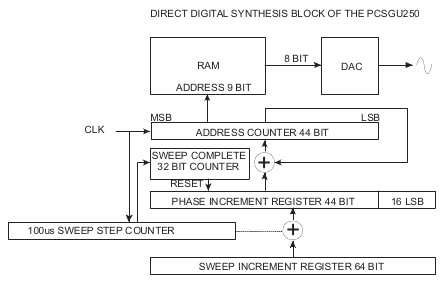
\includegraphics{sweep}
\caption{Общая схема генератора}
\label{gen:plot}
\end{figure}

\subsubsection{Элементы}
В генераторе используется несколько основных элементов:
\begin{itemize}
\item \texttt{RAM}: 9-битное оперативное запоминающее устройство. При установке на его
  входы 9-битного адреса устанавливает на своих выходах значение байта по этому
  адресу.
\item \texttt{ADDRESS COUNTER}: 44-битный счётчик адреса. Его верхние 9 бит
  служат адресом для \texttt{RAM}. Таким образом реализовано округление числа с
  фиксированной запятой.
\item \texttt{DAC}: Аналого-цифровой преобразователь. На основе настроек
  генератора и поступающего на его вход 8-битного значения устанавливает
  напряжение на своём выходе.
\item \texttt{CLK}: Внешний генератор такта; работает с частотой 12.5 или 6.25
  МГц.
\item \texttt{SWEEP COMPLETE COUNTER}: Каждый такт этот счётчик увеличивается на
  единицу и сбрасывается по достижении определённого значения.
\end{itemize}

\subsubsection{Регистры}
В генераторе используется несколько регистров, задающих его работу:
\begin{itemize}
\item \texttt{PHASE INCREMENT REGISTER}: устанавливает скорость изменения
  выходной точки волны. Каждый такт генератора значение из этого регистра
  прибавляется к значению \texttt{ADDRESS COUNTER}. Таким образом, за некоторое
  количество тактом верхние 9 бит \texttt{ADDRESS COUNTER} увеличатся; так
  реализуется произвольная (до некоторой степени) частота работы генератора.
\item \texttt{SWEEP INCREMENT REGISTER}: устанавливает скорость увеличения
  \texttt{PHASE INCREMENT REGISTER} на каждый такт. Таким образом реализуется
  гребёнка, то есть повышение частоты выходной волны во времени. Также каждый
  такт увеличивается значение счётчика 
\item \texttt{SWEEP COMPLETE REGISTER}: устанавливает верхнюю границу для
  \texttt{SWEEP COMPLETE COUNTER}. Каждый такт значение из этого регистра
  сравнивается со значением \texttt{SWEEP COMPLETE COUNTER}. Если значения
  равны, происходит сброс счётчика, а также регистра \texttt{PHASE INCREMENT
    REGISTER} в начальное состояние. Таким образом реализуется повторяющееся во
  времени гребёнка.
\end{itemize}
Значения этих регистров устанавливаются пользователем; более подробно это
описано в разделе~\ref{configuration_freq}. Реально схема генератора сложнее;
это обусловлено поддержкой логарифмической гребёнки.

\subsection{Выводы}
Драйвер устройства должен быть написан для работы на уровне ядра Linux. Он
должен представлть собой драйвер для конкретного устройства с интерфейсом USB,
не для класса. Он должен работать с устройством по определённому (пока
неисвестному) протоколу. Он должен управлять определёнными характеристиками
устройства, уметь устанавливать регистры для генератора, считывать информацию и
передавать её пользовательской программе.

\newpage
\section{Конструкторский раздел}
\subsection{Протокол работы с осциллографом}
Управление и работа с осциллографом представляет собой обмен командами и данными
через его две конечных точки типа ``прерывание''. Протокол зашит разработчиками
устройства и не подлежит изменениям со стороны драйвера. Этот протокол был
обратно разработан в ходе работы над проектом.

Устройство представляет собой внутри автомат, реагирующий опредённым образом на
входящие управляющие последовательности в зависимости от состояния, и
отправляющий данные в ответ.~\cite{scopespecs} Состояния приведены на
рисунке~\ref{scopestates}. Далее будет рассмотрен каждое из них по-отдельности.

\begin{figure}[h!]
\centering
\begin{dot2tex}[scale=0.8]
digraph pcsgu250_states {
  start [label = "Начало"];
  firmware_load [label = "Загрузка прошивки"];
  ready [label = "Готовность"];
  wave_load [label = "Приём волны"];
  trigger_wait [label = "Ожидание триггера"];
  triggered [label = "Готовность данных"];

  start -> firmware_load [label="Запрос"];
  firmware_load -> ready [label="Загрузка"];
  ready -> ready [label="Настройка/сброс/генерация"];
  ready -> wave_load [label="Отправка волны"];
  wave_load -> ready [label="Конец отправки волны"];
  ready -> trigger_wait [label="Запуск"];
  trigger_wait -> triggered [label="Триггер"];
  triggered -> ready [label="Чтение/малое чтение"];

  overlap = false;
}
\end{dot2tex}
\caption{Граф состояний осциллографа}
\label{scopestates}
\end{figure}

\subsubsection{Начало} \label{ostate:start}
Это состояние устройства после его подключения. \\
Переходы:
\begin{itemize}
\item Запрос: байт \texttt{08} переводит устройство в состояние загрузки
  прошивки.
\end{itemize}

\subsubsection{Загрузка прошивки} \label{ostate:fw}
В этом состоянии устройство ожидает приёма своей прошивки от драйвера. \\
Переходы:
\begin{itemize}
\item Загрузка: пересылка прошивки (версия прошивки 1.01 имеет размер 54912 байт)
\end{itemize}

\subsubsection{Готовность} \label{ostate:ready}
В этом состоянии устройство готово к работе и к приёму своих основных команд. \\
Переходы:
\begin{itemize}
\item Настройка: отправка пакета настройки (будет подробнее рассмотрено
  в~\ref{configuration}) не изменяет основного состояния устройства,
  устанавливая внутренние регистры.
\item Сброс: байт \texttt{09} сбрасывает текущие данные из внутренней памяти
  осциллографа, что позволяет загрузить новые.
\item Генерация: байт \texttt{06} включает генератор волны.
\item Отправка волны: байт \texttt{04} начинает передачу новой волны в
  устройство и переводит его в состояние приёма волны. Также он останавливает
  генерацию волны, если она была включена.
\item Запуск: байт \texttt{0B} включает триггер и начинает измерение входных
  данных, переводя устройство в состояние ожидания триггера.
\end{itemize}

\subsubsection{Приём волны} \label{ostate:wave}
В этом состоянии осциллограф ожидает пакета размером 512 байт с точками,
задающими период волны для генератора. \\
Переходы:
\begin{itemize}
\item Конец отправки волны: после окончания отправки волны устройство
  устанавливает новую волну и переходит в состояние готовности.
\end{itemize}

\subsubsection{Ожидание триггера} \label{ostate:trigger}
В этом состоянии осциллограф дожидается срабатывания триггера, а затем
производит измерения с входных каналов пока буфер не будет заполнен. Во время
ожидания осциллограф непрерывно посылает байт \texttt{4E}. К сожалению, в
программе устройства есть ошибка, из-за которой оно иногда перед отправкой
первого байта \texttt{4E} посылает 64 байта мусорных данных. После общения с
разработчиками оказалось, что эта ошибка известна и её тяжело предсказать. В
такой ситуации если считывать из USB 1 байт, то наступает переполнение
буфера. Если же считывать 64 байта, то драйвер будет находиться в вечном
ожидании данных от устройства. После изучения ошибки было замечено, что
осциллограф обычно не проявляет эту ошибку сразу после настройки, но проявляет
каждый последующий раз. Таким образом, перед вторым и следующими ожиданиями
триггера после настройки драйвер должен считать 64 байта мусорных данных. Это не
всегда работает, и в драйвере предусмотрены как таймаут для ожидания 64 байт,
так и обработка ошибки переполнения буфера, в случае которой осциллограф
возвращается в состояние готовности.

После окончания ожидания и записи данных во внутренний буфер осциллограф
посылает байт \texttt{44} и переходит в состояние готовности данных.

\subsubsection{Готовность данных} \label{ostate:data}
В этом состоянии осциллограф ожидает чтения измеренных величин из своего
буфера. \\
Переходы:
\begin{itemize}
\item Чтение: байт \texttt{0A} запрашивает у осциллографа 8192 байта данных. Из
  них первый байт --- это первое измерение для первого канала, второй --- первое
  для второго, третий --- второе для первого и.т.д.
\item Малое чтение: байт \texttt{0C} запрашивает у осциллографа 64 байта
  данных. Данные располагаются в таком же формате. Малое чтение используется для
  режима осциллографа, в котором он отправляет данные раз за разом крайне
  быстро, что используется для записи редких импульсов.
\end{itemize}
После отправки всех данных осциллограф переходит в состояние готовности.


\subsection{Конфигурация} \label{configuration}
Для конфигурации осциллографа используется специальный формат пакетов, который
будет здесь рассмотрел вместе с возможными параметрами конфигурации устройства.

\subsubsection{Конфигурация осциллографа}
Для конфигурации осциллографа используется пакет размером в 10 байт. Формат
пакета приведён в листинге~\ref{conf:scope}. Ниже будут рассмотрены все
параметры конфигурации осциллографа.

\begin{lstlisting}[language=,float=h!,caption={Пакет настройки
  осциллографа},label=conf:scope]
0x0E
0x80
0x07
$\text{volt\_div}_1$ + $\text{DC\_coupling}_1$ + ($\text{GND\_coupling}_1$ << 4)
$\text{volt\_div}_2$ + $\text{DC\_coupling}_2$ + ($\text{GND\_coupling}_2$ << 4)
$\text{y\_position}_1$
$\text{y\_position}_2$
$\text{trigg\_level}$
$\text{time\_div}$
$\text{trg\_ch}$ + ($\text{no\_trg}$ << 1) + ($\text{neg\_trg}$ << 2) +($\text{digi\_on}$ << 3)
\end{lstlisting}

\begin{itemize}
\item $\text{volt\_div}_i$: возможное максимальное напряжение для канала. Чем
  ниже, тем больше точность измерения в пределах этой величины. Возможные
  значения приведены в таблице~\ref{conf:scope:volt}.

\begin{table}[h!]
\centering
\begin{tabu} {|l|l|}
\hline
Байт & Напряжение \\ \hline
\texttt{22} & 10 мВ \\ \hline
\texttt{02} & 30 мВ \\ \hline
\texttt{24} & 0.1 В \\ \hline
\texttt{04} & 0.3 В \\ \hline
\texttt{28} & 1 В \\ \hline
\texttt{08} & 3 В \\ \hline
\end{tabu}
\caption{Возможные параметры $\text{volt\_div}_i$}
\label{conf:scope:volt}
\end{table}

\item $\text{DC\_coupling}$: установить для данного канала связь на постоянный
  ток (0 или 1). Эта опция не может быть установлена одновременно с
  $\text{GND\_coupling}_i$. Если ни одна из этих опций не установлена, считается
  что включена связь на переменный ток.
\item $\text{GND\_coupling}_i$: установить для данного канала связь на землю (0
  или 1). Эта опция не может быть установлена одновременно с
  $\text{DC\_coupling}_i$. Если ни одна из этих опций не установлена, считается
  что включена связь на переменный ток.
\item $\text{y\_position}_i$: Величина отступа для канала, байт. Это напряжение
  прибавляется к входному перед снятием значения. Среднее значение (измеренное
  производителем) составляет \texttt{78}, минимальное --- \texttt{00},
  максимальное --- \texttt{F7}.
\item $\text{trigg\_level}$: Уровень срабатывания триггера, байт. Это
  напряжение, на котором сработает встроенный триггер.
\item $\text{time\_div}$: Частота осциллографа. Возможные значения приведены в
  таблице~\ref{conf:scope:time}.

\begin{table}[h!]
\centering
\begin{tabu} {|l|l|}
\hline
Байт & Частота \\ \hline
\texttt{C1} & 250 Гц \\ \hline
\texttt{C2} & 625 Гц \\ \hline
\texttt{E0} & 1.25 кГц \\ \hline
\texttt{E1} & 2.5 кГц \\ \hline
\texttt{E2} & 6.25 кГц \\ \hline
\texttt{F0} & 12.5 кГц \\ \hline
\texttt{F1} & 25 кГц \\ \hline
\texttt{F2} & 62.5 кГц \\ \hline
\texttt{F8} & 125 кГц \\ \hline
\texttt{F9} & 250 кГц \\ \hline
\texttt{FA} & 625 кГц \\ \hline
\texttt{FC} & 1.25 МГц \\ \hline
\texttt{FD} & 2.5 МГц \\ \hline
\texttt{FE} & 6.25 МГц \\ \hline
\texttt{80} & 12.5 МГц \\ \hline
\texttt{40} & 25 МГц \\ \hline
\texttt{02} & 12.5 МГц (запись внезапных сигналов) \\ \hline
\end{tabu}
\caption{Возможные параметры $\text{time\_div}$}
\label{conf:scope:time}
\end{table}

\item $\text{no\_trg}$: состояние триггера (0 или 1). Если бит установлен, то
  триггер включён и запись данных будет вестить по его активации.
\item $\text{neg\_trg}$: направление триггера (0 или 1). Если бит установлен, то
  триггер срабатывает, когда входная волна проходит установленное напряжение при
  понижении амплитуды, если снят, то когда волна проходит напряжение при
  повышении.
\item $\text{digi\_on}$: цифровой режим (0 или 1). Если бит установлен, то
  осциллограф возвращает результат измерения цифрового сигнала. Это бывает
  удобно для изучения работы цифровых контуров. (хотя, в целом, может быть
  реализовано программно)
\end{itemize}
Собранный таким образом пакет отправляется осциллографу в состоянии готовности.

\subsubsection{Конфигурация генератора}
Для конфигурации генератора используется пакет размером в 7 байт. Формат
пакета приведён в листинге~\ref{conf:gen}. Ниже будут рассмотрены все
параметры конфигурации генератора.

\begin{lstlisting}[language=,float=h!,caption={Пакет настройки
  генератора},label=conf:gen]
0x0E
0x05
0x04
$\text{dc\_offset}$
$\text{ampl}$ + ($\text{sel\_f}$ << 3) + ($\text{relay\_state}$ << 64)
$\text{correction}$ + ($\text{power\_LED}$ << 4)
$\text{filter}$ + ($\text{enable\_sweep}$ << 3)
\end{lstlisting}

\begin{itemize}
\item $\text{dc\_offset}$: отступ волны, байт. Нулевой отступ достигается при
  значении \texttt{7F}, отступ в -5 В при \texttt{00} и в +5 В при \texttt{FF}.
\item $\text{ampl}$: амплитуда выходного сигнала, 3 бита.
\item $\text{sel\_f}$: диапазон частот осциллографа, 3 бита. Не поддерживается
  текущей версией встроенного ПО и должен быть равен \texttt{00}.
\item $\text{relay\_state}$: состояние реле генератора, 2 бита. Не поддерживается
  текущей версией встроенного ПО и должен быть равен \texttt{00}.
\item $\text{correction}$: поправка амплитуды, 3 бита. Среднее значение ---
  \texttt{04}, используется для улучшения формы волны в некоторых случаях.
\item $\text{power\_LED}$: состояние светодиода осциллографа, 2 бита. Возможные
  состояния приведены в таблице~\ref{conf:gen:led}.

\begin{table}[h!]
\centering
\begin{tabu} {|l|l|}
\hline
Байт & Состояние светодиода \\ \hline
\texttt{00} & Выключен \\ \hline
\texttt{01} & Умеренно горит \\ \hline
\texttt{02} & Сильно горит \\ \hline
\end{tabu}
\caption{Возможные параметры $\text{power\_LED}$}
\label{conf:gen:led}
\end{table}

\item $\text{filter}$: Установка фильтра генератора, 3 бита. Внутренний фильтр
  генератора влияет на форму и качество конечного сигнала. Рекомендуемые
  значения фильтра от разработчика приведены в таблице~\ref{conf:gen:filter}.
  Дополнительным свойством этого параметра является установка частоты
  генератора. При значении $\text{filter} > 5$ частота составляет 6.25 МГц,
  иначе 12.5 МГц.

\begin{table}[h!]
\centering
\begin{tabu} {|l|l|l|}
\hline
Тип волны & Частота & Байт \\ \hline
\multirow{6}{*}{Гребёнка} & 0..50 кГц & \texttt{07} \\
 & 50..150 кГц & \texttt{06} \\
 & 150..300 кГц & \texttt{05} \\
 & 300..500 кГц & \texttt{04} \\
 & 500..700 кГц & \texttt{02} \\
 & 700..1000 кГц & \texttt{01} \\ \hline
\multirow{6}{*}{$\sin(x)$} & 0..50 кГц & \texttt{07} \\
 & 50..150 кГц & \texttt{06} \\
 & 150..300 кГц & \texttt{05} \\
 & 300..400 кГц & \texttt{03} \\
 & 400..500 кГц & \texttt{02} \\
 & 500..1000 кГц & \texttt{01} \\ \hline
\multirow{3}{*}{$\sin(x)/x$} & 0..5 кГц & \texttt{07} \\
 & 5..50 кГц & \texttt{06} \\
 & 50..500 кГц & \texttt{01} \\ \hline
Прямоугольная & Любая & \texttt{00} \\ \hline
Константа & - & \texttt{07} \\ \hline
\multirow{2}{*}{Другая} & 0..50 кГц & \texttt{07} \\
 & 50..500 кГц & \texttt{00} \\ \hline
\end{tabu}
\caption{Рекомендуемые значения $\text{filter}$}
\label{conf:gen:filter}
\end{table}

\item $\text{enable\_sweep}$: этот параметр включает или отключает работу
  регистров смещения генератора. Реально он отключает какие-либо изменения
  регистров генератора, так что если этот бит сброшен, генератор неактивен.
\end{itemize}

\subsubsection{Конфигурация регистров генератора} \label{configuration_freq}
Для конфигурации регистров генератора используется пакет размером в 22
байта. Формат пакета приведён в листинге~\ref{conf:freq}. Ниже будут
рассмотрены формулы для расчётов соответствующих регистров.

\begin{lstlisting}[language=,float=h!,caption={Пакет настройки
  регистров генератора},label=conf:freq]
0x0E
0x02
0x13
SWEEP INCREMENT REGISTER, 8 байт
-
-
-
-
-
-
$\text{Старший байт}$
PHASE INCREMENT REGISTER, 6 байт
-
-
-
-
$\text{Старший байт}$
SWEEP COMPLETE REGISTER, 5 байт
-
-
-
$\text{Старший байт; бит логарифмической гребёнки}$
\end{lstlisting}

\begin{itemize}
\item \texttt{SWEEP INCREMENT REGISTER}: расчитывается по формуле:
\begin{equation}
2^a \frac{\nu_2 - \nu_1}{\nu \cdot t}
\end{equation}
, где $a$ расчитывается так: к числу 60 прибавляется 4 если гребёнка будет
линейной, и 1 если частота равна 6.25 МГц. $nu_2$ и $nu_1$ --- конечная и
начальная частоты для гребёнки соответственно (если гребёнку нужно выключить,
начальная и конечная частоты равны). $\nu$ --- частота генератора, а $t$ ---
желаемое время периода возрастания гребёнки в промежутках по 100 мкс.
\item \texttt{PHASE INCREMENT REGISTER}: расчитывается по формуле:
\begin{equation}
2^{44} \frac{\nu_1}{\nu}
\end{equation}
, где $\nu_1$ --- желаемая начальная частота генератора, а $\nu$ --- частота
генератора.
\item \texttt{SWEEP COMPLETE REGISTER}: расчитывается по формуле:
\begin{equation}
\frac{t}{a} + b
\end{equation}
, где $t$ --- желаемое время периода возрастания гребёнки, $a$ --- 1, если
гребёнка линейная или 8, если логарифмическая, и делится на 2, если частота
равна 6.25 МГц. $b$ --- 0, если необходима линейная, или 2 --- если
логарифмическая гребёнка.
\end{itemize}

\subsubsection{Процесс работы}
Процесс работы с модулем предполагался следующий:
\begin{enumerate}
\item Пользователь подключает осциллограф к компьютеру, он инициализируется в
  фоне и в него загружается микропрограмма.
\item После загрузки устройство готово к работе и пользователь может
  использовать различные вызовы.
\item После вызова \texttt{SIO\_TRIGGER} приложение блокируется до готовности
  осциллографа к отправке данных. Это было запланированно чтобы дать
  пользователю возможность сохранить момент времени в который осциллограф
  сообщил о готовности, для отображения на графике.
\item Вызов \texttt{SIO\_TRIGGER} в фоне запускает процесс чтения данных с
  осциллографа. При вызове \texttt{read()} в момент между началом и окончанием
  чтения данных с устройства, вызов блокируется по желанию пользователя до
  окончания чтения из устройства в буфер.
\item После окончания чтения из устройства оно снова готово к работе, а данные
  содержаться в буфере и считываются при помощи \texttt{read()}.
\end{enumerate}
Такой подход прост и удобен для проектировщика пользовательского приложения, а
также раскрывает все возможности осциллографа и даёт возможность использовать
неблокирующие вызовы там, где это имеет смысл.

\subsection{Точки входа}
Общая схема взаимодействия модуля, устройства и пользовательской программы
приведена на рисунке~\ref{interaction}.

\begin{figure}[h!]
\centering
% Graphic for TeX using PGF
% Title: /home/abbradar/Диаграмма1.dia
% Creator: Dia v0.97.2
% CreationDate: Mon May 27 14:49:30 2013
% For: abbradar
% \usepackage{tikz}
% The following commands are not supported in PSTricks at present
% We define them conditionally, so when they are implemented,
% this pgf file will use them.
\ifx\du\undefined
  \newlength{\du}
\fi
\setlength{\du}{15\unitlength}
\begin{tikzpicture}
\pgftransformxscale{1.000000}
\pgftransformyscale{-1.000000}
\definecolor{dialinecolor}{rgb}{0.000000, 0.000000, 0.000000}
\pgfsetstrokecolor{dialinecolor}
\definecolor{dialinecolor}{rgb}{1.000000, 1.000000, 1.000000}
\pgfsetfillcolor{dialinecolor}
% setfont left to latex
\definecolor{dialinecolor}{rgb}{0.000000, 0.000000, 0.000000}
\pgfsetstrokecolor{dialinecolor}
\node[anchor=west] at (12.000000\du,32.000000\du){};
\definecolor{dialinecolor}{rgb}{1.000000, 1.000000, 1.000000}
\pgfsetfillcolor{dialinecolor}
\fill (17.000000\du,29.000000\du)--(17.000000\du,32.000000\du)--(23.000000\du,32.000000\du)--(23.000000\du,29.000000\du)--cycle;
\pgfsetlinewidth{0.100000\du}
\pgfsetdash{}{0pt}
\pgfsetdash{}{0pt}
\pgfsetmiterjoin
\definecolor{dialinecolor}{rgb}{0.000000, 0.000000, 0.000000}
\pgfsetstrokecolor{dialinecolor}
\draw (17.000000\du,29.000000\du)--(17.000000\du,32.000000\du)--(23.000000\du,32.000000\du)--(23.000000\du,29.000000\du)--cycle;
% setfont left to latex
\definecolor{dialinecolor}{rgb}{0.000000, 0.000000, 0.000000}
\pgfsetstrokecolor{dialinecolor}
\node at (20.000000\du,30.700000\du){Драйвер};
\pgfsetlinewidth{0.100000\du}
\pgfsetdash{}{0pt}
\pgfsetdash{}{0pt}
\pgfsetbuttcap
\pgfsetmiterjoin
\pgfsetlinewidth{0.100000\du}
\pgfsetbuttcap
\pgfsetmiterjoin
\pgfsetdash{}{0pt}
\definecolor{dialinecolor}{rgb}{0.000000, 0.000000, 0.000000}
\pgfsetstrokecolor{dialinecolor}
\draw (7.000000\du,29.000000\du)--(7.000000\du,32.000000\du);
\pgfsetbuttcap
\pgfsetmiterjoin
\pgfsetdash{}{0pt}
\definecolor{dialinecolor}{rgb}{0.000000, 0.000000, 0.000000}
\pgfsetstrokecolor{dialinecolor}
\draw (7.000000\du,29.000000\du)--(12.326316\du,29.000000\du);
\pgfsetbuttcap
\pgfsetmiterjoin
\pgfsetdash{}{0pt}
\definecolor{dialinecolor}{rgb}{0.000000, 0.000000, 0.000000}
\pgfsetstrokecolor{dialinecolor}
\draw (7.000000\du,32.000000\du)--(12.326316\du,32.000000\du);
% setfont left to latex
\definecolor{dialinecolor}{rgb}{0.000000, 0.000000, 0.000000}
\pgfsetstrokecolor{dialinecolor}
\node at (9.796316\du,30.775000\du){Осциллограф};
\pgfsetlinewidth{0.100000\du}
\pgfsetdash{}{0pt}
\pgfsetdash{}{0pt}
\pgfsetbuttcap
{
\definecolor{dialinecolor}{rgb}{0.000000, 0.000000, 0.000000}
\pgfsetfillcolor{dialinecolor}
% was here!!!
\pgfsetarrowsend{stealth}
\definecolor{dialinecolor}{rgb}{0.000000, 0.000000, 0.000000}
\pgfsetstrokecolor{dialinecolor}
\draw (12.326316\du,29.750000\du)--(17.000000\du,29.750000\du);
}
\pgfsetlinewidth{0.100000\du}
\pgfsetdash{}{0pt}
\pgfsetdash{}{0pt}
\pgfsetbuttcap
{
\definecolor{dialinecolor}{rgb}{0.000000, 0.000000, 0.000000}
\pgfsetfillcolor{dialinecolor}
% was here!!!
\pgfsetarrowsend{stealth}
\definecolor{dialinecolor}{rgb}{0.000000, 0.000000, 0.000000}
\pgfsetstrokecolor{dialinecolor}
\draw (17.000000\du,31.250000\du)--(12.326316\du,31.250000\du);
}
\pgfsetlinewidth{0.100000\du}
\pgfsetdash{}{0pt}
\pgfsetdash{}{0pt}
\pgfsetbuttcap
\pgfsetmiterjoin
\pgfsetlinewidth{0.100000\du}
\pgfsetbuttcap
\pgfsetmiterjoin
\pgfsetdash{}{0pt}
\definecolor{dialinecolor}{rgb}{1.000000, 1.000000, 1.000000}
\pgfsetfillcolor{dialinecolor}
\pgfpathmoveto{\pgfpoint{27.050000\du}{29.066667\du}}
\pgfpathcurveto{\pgfpoint{28.250000\du}{28.566667\du}}{\pgfpoint{28.850000\du}{28.400000\du}}{\pgfpoint{30.050000\du}{28.400000\du}}
\pgfpathcurveto{\pgfpoint{31.250000\du}{28.400000\du}}{\pgfpoint{31.850000\du}{28.566667\du}}{\pgfpoint{33.050000\du}{29.066667\du}}
\pgfpathlineto{\pgfpoint{33.050000\du}{31.733333\du}}
\pgfpathcurveto{\pgfpoint{31.850000\du}{32.233333\du}}{\pgfpoint{31.250000\du}{32.400000\du}}{\pgfpoint{30.050000\du}{32.400000\du}}
\pgfpathcurveto{\pgfpoint{28.850000\du}{32.400000\du}}{\pgfpoint{28.250000\du}{32.233333\du}}{\pgfpoint{27.050000\du}{31.733333\du}}
\pgfpathlineto{\pgfpoint{27.050000\du}{29.066667\du}}
\pgfusepath{fill}
\definecolor{dialinecolor}{rgb}{0.000000, 0.000000, 0.000000}
\pgfsetstrokecolor{dialinecolor}
\pgfpathmoveto{\pgfpoint{27.050000\du}{29.066667\du}}
\pgfpathcurveto{\pgfpoint{28.250000\du}{28.566667\du}}{\pgfpoint{28.850000\du}{28.400000\du}}{\pgfpoint{30.050000\du}{28.400000\du}}
\pgfpathcurveto{\pgfpoint{31.250000\du}{28.400000\du}}{\pgfpoint{31.850000\du}{28.566667\du}}{\pgfpoint{33.050000\du}{29.066667\du}}
\pgfpathlineto{\pgfpoint{33.050000\du}{31.733333\du}}
\pgfpathcurveto{\pgfpoint{31.850000\du}{32.233333\du}}{\pgfpoint{31.250000\du}{32.400000\du}}{\pgfpoint{30.050000\du}{32.400000\du}}
\pgfpathcurveto{\pgfpoint{28.850000\du}{32.400000\du}}{\pgfpoint{28.250000\du}{32.233333\du}}{\pgfpoint{27.050000\du}{31.733333\du}}
\pgfpathlineto{\pgfpoint{27.050000\du}{29.066667\du}}
\pgfusepath{stroke}
\pgfsetbuttcap
\pgfsetmiterjoin
\pgfsetdash{}{0pt}
\definecolor{dialinecolor}{rgb}{0.000000, 0.000000, 0.000000}
\pgfsetstrokecolor{dialinecolor}
\pgfpathmoveto{\pgfpoint{27.050000\du}{29.066667\du}}
\pgfpathcurveto{\pgfpoint{28.250000\du}{29.566667\du}}{\pgfpoint{28.850000\du}{29.733333\du}}{\pgfpoint{30.050000\du}{29.733333\du}}
\pgfpathcurveto{\pgfpoint{31.250000\du}{29.733333\du}}{\pgfpoint{31.850000\du}{29.566667\du}}{\pgfpoint{33.050000\du}{29.066667\du}}
\pgfusepath{stroke}
% setfont left to latex
\definecolor{dialinecolor}{rgb}{0.000000, 0.000000, 0.000000}
\pgfsetstrokecolor{dialinecolor}
\node at (30.050000\du,30.933333\du){Файл ядра};
\pgfsetlinewidth{0.100000\du}
\pgfsetdash{{1.000000\du}{1.000000\du}}{0\du}
\pgfsetdash{{1.000000\du}{1.000000\du}}{0\du}
\pgfsetbuttcap
{
\definecolor{dialinecolor}{rgb}{0.000000, 0.000000, 0.000000}
\pgfsetfillcolor{dialinecolor}
% was here!!!
\definecolor{dialinecolor}{rgb}{0.000000, 0.000000, 0.000000}
\pgfsetstrokecolor{dialinecolor}
\draw (34.000000\du,25.000000\du)--(6.000000\du,25.000000\du);
}
% setfont left to latex
\definecolor{dialinecolor}{rgb}{0.000000, 0.000000, 0.000000}
\pgfsetstrokecolor{dialinecolor}
\node[anchor=west] at (17.000000\du,26.000000\du){Уровень ядра};
% setfont left to latex
\definecolor{dialinecolor}{rgb}{0.000000, 0.000000, 0.000000}
\pgfsetstrokecolor{dialinecolor}
\node[anchor=west] at (17.000000\du,24.000000\du){Уровень задачи};
\pgfsetlinewidth{0.100000\du}
\pgfsetdash{}{0pt}
\pgfsetdash{}{0pt}
\pgfsetbuttcap
{
\definecolor{dialinecolor}{rgb}{0.000000, 0.000000, 0.000000}
\pgfsetfillcolor{dialinecolor}
% was here!!!
\pgfsetarrowsend{stealth}
\definecolor{dialinecolor}{rgb}{0.000000, 0.000000, 0.000000}
\pgfsetstrokecolor{dialinecolor}
\draw (23.000000\du,31.250000\du)--(27.088197\du,31.250000\du);
}
\pgfsetlinewidth{0.100000\du}
\pgfsetdash{}{0pt}
\pgfsetdash{}{0pt}
\pgfsetbuttcap
{
\definecolor{dialinecolor}{rgb}{0.000000, 0.000000, 0.000000}
\pgfsetfillcolor{dialinecolor}
% was here!!!
\pgfsetarrowsend{stealth}
\definecolor{dialinecolor}{rgb}{0.000000, 0.000000, 0.000000}
\pgfsetstrokecolor{dialinecolor}
\draw (27.050000\du,29.766667\du)--(23.000000\du,29.750000\du);
}
\definecolor{dialinecolor}{rgb}{1.000000, 1.000000, 1.000000}
\pgfsetfillcolor{dialinecolor}
\fill (27.000000\du,19.000000\du)--(27.000000\du,21.800000\du)--(33.000000\du,21.800000\du)--(33.000000\du,19.000000\du)--cycle;
\pgfsetlinewidth{0.100000\du}
\pgfsetdash{}{0pt}
\pgfsetdash{}{0pt}
\pgfsetmiterjoin
\definecolor{dialinecolor}{rgb}{0.000000, 0.000000, 0.000000}
\pgfsetstrokecolor{dialinecolor}
\draw (27.000000\du,19.000000\du)--(27.000000\du,21.800000\du)--(33.000000\du,21.800000\du)--(33.000000\du,19.000000\du)--cycle;
% setfont left to latex
\definecolor{dialinecolor}{rgb}{0.000000, 0.000000, 0.000000}
\pgfsetstrokecolor{dialinecolor}
\node at (30.000000\du,20.200000\du){Программа};
% setfont left to latex
\definecolor{dialinecolor}{rgb}{0.000000, 0.000000, 0.000000}
\pgfsetstrokecolor{dialinecolor}
\node at (30.000000\du,21.000000\du){пользователя};
\pgfsetlinewidth{0.100000\du}
\pgfsetdash{}{0pt}
\pgfsetdash{}{0pt}
\pgfsetbuttcap
{
\definecolor{dialinecolor}{rgb}{0.000000, 0.000000, 0.000000}
\pgfsetfillcolor{dialinecolor}
% was here!!!
\pgfsetarrowsend{stealth}
\definecolor{dialinecolor}{rgb}{0.000000, 0.000000, 0.000000}
\pgfsetstrokecolor{dialinecolor}
\draw (28.100000\du,28.650000\du)--(28.100000\du,21.650000\du);
}
\pgfsetlinewidth{0.100000\du}
\pgfsetdash{}{0pt}
\pgfsetdash{}{0pt}
\pgfsetbuttcap
{
\definecolor{dialinecolor}{rgb}{0.000000, 0.000000, 0.000000}
\pgfsetfillcolor{dialinecolor}
% was here!!!
\pgfsetarrowsend{stealth}
\definecolor{dialinecolor}{rgb}{0.000000, 0.000000, 0.000000}
\pgfsetstrokecolor{dialinecolor}
\draw (31.950000\du,21.800000\du)--(31.950000\du,28.800000\du);
}
\pgfsetlinewidth{0.100000\du}
\pgfsetdash{}{0pt}
\pgfsetdash{}{0pt}
\pgfsetbuttcap
{
\definecolor{dialinecolor}{rgb}{0.000000, 0.000000, 0.000000}
\pgfsetfillcolor{dialinecolor}
% was here!!!
\pgfsetarrowsend{stealth}
\definecolor{dialinecolor}{rgb}{0.000000, 0.000000, 0.000000}
\pgfsetstrokecolor{dialinecolor}
\draw (27.000000\du,20.000000\du)--(23.000000\du,20.000000\du);
}
\definecolor{dialinecolor}{rgb}{1.000000, 1.000000, 1.000000}
\pgfsetfillcolor{dialinecolor}
\fill (17.000000\du,19.000000\du)--(17.000000\du,22.000000\du)--(23.000000\du,22.000000\du)--(23.000000\du,19.000000\du)--cycle;
\pgfsetlinewidth{0.100000\du}
\pgfsetdash{}{0pt}
\pgfsetdash{}{0pt}
\pgfsetmiterjoin
\definecolor{dialinecolor}{rgb}{0.000000, 0.000000, 0.000000}
\pgfsetstrokecolor{dialinecolor}
\draw (17.000000\du,19.000000\du)--(17.000000\du,22.000000\du)--(23.000000\du,22.000000\du)--(23.000000\du,19.000000\du)--cycle;
% setfont left to latex
\definecolor{dialinecolor}{rgb}{0.000000, 0.000000, 0.000000}
\pgfsetstrokecolor{dialinecolor}
\node at (20.000000\du,20.680000\du){};
\pgfsetlinewidth{0.100000\du}
\pgfsetdash{}{0pt}
\pgfsetdash{}{0pt}
\pgfsetbuttcap
\pgfsetmiterjoin
\pgfsetlinewidth{0.100000\du}
\pgfsetbuttcap
\pgfsetmiterjoin
\pgfsetdash{}{0pt}
\definecolor{dialinecolor}{rgb}{1.000000, 1.000000, 1.000000}
\pgfsetfillcolor{dialinecolor}
\pgfpathmoveto{\pgfpoint{18.200000\du}{19.350000\du}}
\pgfpathlineto{\pgfpoint{21.800000\du}{19.350000\du}}
\pgfpathcurveto{\pgfpoint{22.297057\du}{19.350000\du}}{\pgfpoint{22.700000\du}{19.864872\du}}{\pgfpoint{22.700000\du}{20.500000\du}}
\pgfpathcurveto{\pgfpoint{22.700000\du}{21.135128\du}}{\pgfpoint{22.297057\du}{21.650000\du}}{\pgfpoint{21.800000\du}{21.650000\du}}
\pgfpathlineto{\pgfpoint{18.200000\du}{21.650000\du}}
\pgfpathcurveto{\pgfpoint{17.702943\du}{21.650000\du}}{\pgfpoint{17.300000\du}{21.135128\du}}{\pgfpoint{17.300000\du}{20.500000\du}}
\pgfpathcurveto{\pgfpoint{17.300000\du}{19.864872\du}}{\pgfpoint{17.702943\du}{19.350000\du}}{\pgfpoint{18.200000\du}{19.350000\du}}
\pgfusepath{fill}
\definecolor{dialinecolor}{rgb}{0.000000, 0.000000, 0.000000}
\pgfsetstrokecolor{dialinecolor}
\pgfpathmoveto{\pgfpoint{18.200000\du}{19.350000\du}}
\pgfpathlineto{\pgfpoint{21.800000\du}{19.350000\du}}
\pgfpathcurveto{\pgfpoint{22.297057\du}{19.350000\du}}{\pgfpoint{22.700000\du}{19.864872\du}}{\pgfpoint{22.700000\du}{20.500000\du}}
\pgfpathcurveto{\pgfpoint{22.700000\du}{21.135128\du}}{\pgfpoint{22.297057\du}{21.650000\du}}{\pgfpoint{21.800000\du}{21.650000\du}}
\pgfpathlineto{\pgfpoint{18.200000\du}{21.650000\du}}
\pgfpathcurveto{\pgfpoint{17.702943\du}{21.650000\du}}{\pgfpoint{17.300000\du}{21.135128\du}}{\pgfpoint{17.300000\du}{20.500000\du}}
\pgfpathcurveto{\pgfpoint{17.300000\du}{19.864872\du}}{\pgfpoint{17.702943\du}{19.350000\du}}{\pgfpoint{18.200000\du}{19.350000\du}}
\pgfusepath{stroke}
% setfont left to latex
\definecolor{dialinecolor}{rgb}{0.000000, 0.000000, 0.000000}
\pgfsetstrokecolor{dialinecolor}
\node at (20.000000\du,20.700000\du){Экран};
\end{tikzpicture}

\label{interaction}
\caption{Схема взаимодействия}
\end{figure}

\subsubsection{Точки входа}
У всех модулей ядра существует одна или больше точек входа --- мест, в которых
может начаться исполнение модуля ядра. Существует несколько возможных видов
точек входа:
\begin{itemize}
\item Функции инициализации и выгрузки \\
Такие функции (по одной каждого вида на модуль) исполняются при загрузке
модуля. В их роли входит инициализация необходимых полей для работы модуля, его
регистрация в различных подсистемах ядра, возможно запуск одного или нескольких
потоков ядра или вывод сообщений. Например, в случае ядра Linux такие функции
задаются специальными макросами, предоставляемыми заголовками ядра.
\item Функции, вызываемые различными подсистемами \\
Такие функции должны быть предварительно зарегистрированы в соответствующих
подсистемах и вызываются при необходимости обработки какого-либо происходящего в
подсистеме события. Например, подсистема файлов устройств Linux использует
несколько таких функций и вызывает их при системных вызовах чтения, записи или
других операций с файлом данного устройства. Другим примером являются функции
USB-подсистемы, которые вызываются при обнаружении предположительно подходящего
для драйвера устройства или при его отключении.
\item Прерывания \\
Функции, выполняемые в качестве обработчика какого-либо прерывания, также можно
назвать точками входа модуля.
\end{itemize}

\subsubsection{Точки входа из режима ядра}
Драйвер уровня ядра осциллографа регистрируется в различных подсистемах ядра,
добавляя свои обработчики к определённым событиям в системе. Список таких точек
входа по подсистемам приведён в таблице~\ref{entries:kernel}. 

\begin{table}
\centering
\begin{tabu} {|l|l|}
\hline
\multirow{3}{*}{Подсистема USB} & При подключении устройства \\
 & При удалении устройства \\
 & При усыплении и пробуждении устройсва \\ \hline
\multirow{4}{*}{Файл уровня ядра} & При открытии файла \\
 & При закрытии файла \\
 & При чтении из файла \\
 & При вызове \texttt{ioctl()} \\ \hline
\end{tabu}
\label{entries:kernel}
\caption{Точки входа для подсистем ядра}
\end{table}

\subsubsection{Точки входа из режима пользователя}
Драйвер уровня ядра осциллографа также обладает состоянием, хотя упрощённым для
пользователя. Драйвер взяимодействует с пользователем при помощи файлового
устройства, для которого задана операция чтения (получения измерений от
осциллографа) и несколько операций управления, перечисленных в
таблице~\ref{module:ioctls}. Здесь ``тип'' обозначает операцию ввода или вывода:
``R'' --- операция вывода, ``W'' --- ввода, ``R/W'' --- совместно ввода и
вывода, ``-'' --- отсутствие ввода-вывода. Иные операции над устройством
запрещены.

\afterpage{
\begin{landscape}
\begin{table}[h!]
\centering
\begin{tabu} {|l|l|l|l|l|}
\hline
Номер & Название & Тип & Параметр & Назначение \\ \hline
1 & \texttt{SIO\_GET\_VERSION} & R & \texttt{char *} & Получение версии прошивки
\\ \hline
2 & \texttt{SIO\_SCOPE\_SET} & W & \texttt{const struct scope\_settings *} &
Установка настроек осциллографа \\ \hline
3 & \texttt{SIO\_SCOPE\_GET} & R & \texttt{struct scope\_settings *} & Чтение
настроек осциллографа \\ \hline
4 & \texttt{SIO\_GENERATOR\_SET} & W & \texttt{const struct generator\_settings
*} & Установка настроек генератора \\ \hline
5 & \texttt{SIO\_GENERATOR\_GET} & R & \texttt{struct generator\_settings *} &
Чтение настроек генератора \\ \hline
6 & \texttt{SIO\_FREQ\_SET} & W & \texttt{const struct freq\_settings *} &
Установка регистров генератора \\ \hline
7 & \texttt{SIO\_FREQ\_GET} & R & \texttt{struct freq\_settings *} & Чтение
регистров генератора \\ \hline
8 & \texttt{SIO\_WAVEFORM\_SET} & W & \texttt{const unsigned char *} & Установка
волны для генератора \\ \hline
9 & \texttt{SIO\_WAVEFORM\_GET} & R & \texttt{unsigned char *} & Чтение волны
генератора \\ \hline
10 & \texttt{SIO\_TRIGGER} & - & & Запуск триггера \\ \hline
11 & \texttt{SIO\_TIMEDIV\_SIZE} & R & \texttt{size\_t *} & Получение размера
таблицы частот \\ \hline
12 & \texttt{SIO\_TIMEDIV} & R & \texttt{\_\_u32 *} & Получение таблицы частот
\\ \hline
11 & \texttt{SIO\_VOLTDIV\_SIZE} & R & \texttt{size\_t *} & Получение размера
таблицы частот \\ \hline
12 & \texttt{SIO\_VOLTDIV} & R & \texttt{\_\_u32 *} & Получение таблицы
напряжений \\ \hline
\end{tabu}
\caption{Управляющие вызовы драйвера устройства}
\label{module:ioctls}
\end{table}
\end{landscape}
}

\subsection{Выводы}
Драйвер устройства должен поддерживать заданный протокол для работы с
устройством. Он должен поддерживать конфигурирование устройства, отправку
пакетов настройки, а также следить за состоянием устройства. Драйвер должен
обладать заданным нами набором точек входа, и предоставлять по запросу
пользователя необходимые данные. Драйвер должен иметь возможность считывания
данных с осциллографа и должен проверять входящие в него данные настройки на
корректность, а вызываемые действия --- на применимость.

\newpage
\section{Технологический раздел}
Модуль ядра разрабатывался для версии ядра \texttt{Linux 3.9}, с использованием
нескольких подсистем ядра.

\subsection{Структуры и типы данных}
\subsubsection{Состояние}
Состояние драйвера представляет из себя набор битовых флагов:
\begin{itemize}
\item \texttt{SCOPE\_INIT}: установлен, если осциллограф инициализирован.
\item \texttt{SCOPE\_READY}: установлен, если осциллограф в состоянии готовности.
\item \texttt{SCOPE\_TRIGGERING}: установлен, если осциллограф находится в
  состоянии ожидания триггера.
\end{itemize}
Такой набор состояний позволяет удобно определять, какие операции сейчас
возможно производить. Например, до окончания инициализации запрещается считывать
версию прошивки устройства, а большинство операций по установке настроек нельзя
производить пока осциллограф занят. Необходимые состояния для каждого вызова
приведены в таблице~\ref{module:states}.

\begin{table}[h!]
\begin{tabu} {|l|l|}
\hline
Название & Необходимое состояние \\ \hline
\texttt{SIO\_GET\_VERSION} & \texttt{SCOPE\_INIT} \\ \hline
\texttt{SIO\_SCOPE\_SET} & \texttt{SCOPE\_READY} \\ \hline
\texttt{SIO\_SCOPE\_GET} & \texttt{SCOPE\_INIT} \\ \hline
\texttt{SIO\_GENERATOR\_SET} & \texttt{SCOPE\_READY} \\ \hline
\texttt{SIO\_GENERATOR\_GET} & \texttt{SCOPE\_INIT} \\ \hline
\texttt{SIO\_FREQ\_SET} & \texttt{SCOPE\_READY} \\ \hline
\texttt{SIO\_FREQ\_GET} & \texttt{SCOPE\_INIT} \\ \hline
\texttt{SIO\_WAVEFORM\_SET} & \texttt{SCOPE\_READY} \\ \hline
\texttt{SIO\_WAVEFORM\_GET} & \texttt{SCOPE\_INIT} \\ \hline
\texttt{SIO\_TRIGGER} & \texttt{SCOPE\_READY} \\ \hline
\texttt{SIO\_TIMEDIV\_SIZE} & - \\ \hline
\texttt{SIO\_TIMEDIV} & - \\ \hline
\texttt{SIO\_VOLTDIV\_SIZE} & - \\ \hline
\texttt{SIO\_VOLTDIV} & - \\ \hline
\texttt{read()} & \texttt{SCOPE\_READY || SCOPE\_TRIGGERING} \\ \hline
\end{tabu}
\caption{Необходимые состояния для вызовов}
\label{module:states}
\end{table}

\subsubsection{Структуры}
Заголовочные файлы для модуля описывают несколько структур, в которых хранятся и
передаются настройки для различных компонентов осциллографа. Структура для
хранения настроек осциллографа представлена в листинге~\ref{struct:scope}, для
настроек генератора --- в листинге~\ref{struct:gen}, а для регистров генератора
--- в листинге~\ref{struct:freq}.

\begin{lstlisting}[float=h!,label=struct:scope,caption={Структуры параметров
    осциллографа}]
enum coupling_type {
  SCOPE_COUPLING_AC = 0,
  SCOPE_COUPLING_DC = 1,
  SCOPE_COUPLING_GND = 1 << 4,
};

enum trigger_dir {
  TRIGGER_UP = 0 << 2,
  TRIGGER_DOWN = 1 << 2,
};

struct channel_settings {
  unsigned volt_div;
  enum coupling_type coupling;
  __s8 y_pos;
};

struct scope_settings {
  struct channel_settings channel[2];
  __u8 trigg_level;
  unsigned long time_div;
  bool enable_trg;
  __u8 trg_ch;
  enum trigger_dir trg_dir;
  bool digi;
};
\end{lstlisting}

\begin{lstlisting}[float=h!,label=struct:gen,caption={Структура параметров
    генератора}]
enum power_led {
  POWER_LED_OFF = 0 << 4,
  POWER_LED_DIM = 1 << 4,
  POWER_LED_BRIGHT = 2 << 4,
};

struct generator_settings {
  __s16 dc_offset;
  __u8 ampl;
  __s8 correction;
  enum power_led power_led;
  __u8 filter;
  bool enable;
};
\end{lstlisting}

\begin{lstlisting}[float=h!,label=struct:freq,caption={Структура регистров
    генератора}]
enum sweep_type {
  SWEEP_LINEAR = 0,
  SWEEP_LOG = ((__u64)1 << 33),
};

struct freq_settings {
  __u32 start_freq;
  __u32 end_freq;
  __u32 sweep_time;
  bool log_sweep;
};
\end{lstlisting}

Различия этих структур данных от данных в их представлении в пакетах настроек
следующие:
\begin{itemize}
\item Структуризация. Например, для каждого канала осциллографа определа
  отдельная структура, а все параметры выделены в перечислимые типы или битовые
  поля.
\item Знаковость. Там где это возможно, беззнаковые типы для настройки, для
  которых указывалось ``среднее значение'', были заменены на знаковые типы,
  которые соответственно преобразуются самим модулем.
\item Изменённые поля. Отсутсвуют поля, которые не поддерживаются в текущей
  версии встроенного ПО. Кроме того, поле \texttt{enable\_sweep} теперь названо
  \texttt{enable} и отвечает за общее состояние генератора.
\end{itemize}

\subsubsection{Возможные ошибки}
Все вызовы к модулю возвращают 0 (или количество прочитанных байт в случае
\texttt{read()}). Если текущее состояние устройства не позволяет выполнить
вызов, возвращается \texttt{-EBUSY}. Иначе возвращается код ошибки того вызова в
процедуре, который первый вернул ошибку. В случае ошибок по возможности
состояние осциллографа откатывается к предыдущему с сохранением максимально
возможного количества старых настроек.

\subsubsection{Синхронность выполнения вызовов}
Все вызовы к модулю синхронны и возвращают в момент окончания
работы. Исключение составляет вызов \texttt{SIO\_TRIGGER}, который после
окончания работы в фоновом режиме принимает данные от осциллографа. Если
\texttt{read()} был вызван слишком быстро, он блокируется до получения ответа от
осциллографа. Этот вызов также поддерживает флаг \texttt{IO\_NONBLOCK}, с помощью
которого можно отказаться от блокировки. Кроме того, с модуль предполагает
безопасную работу с осциллографом в многопоточном режиме и из разных приложений.

\subsubsection{Доступ к таблицам соответствия}
В состав драйвера входят внутренние таблицы для сопоставления числовых значений
частот и напряжений и соответствующих им байтов для настройки. По специальным
запросам эти таблицы могут быть получены в пользовательской программе. Однако, в
состав драйвера не входят рекомендованные значения фильтра. Предполагается что
это значение должна выставлять сама программа в соответствии с замыслом
программиста.

\subsection{Исследование осциллографа}
Для исследования осциллографа применялось несколько методов. Во-первых, под
виртуальной машиной qemu была установлена ОС Microsoft Windows XP, на которую
было установлено оригинальное программное обеспечение для осциллографа и пробная
версия программи USBlyzer (рисунок~\ref{usblyzer}), которая представляет собой
перехватчик USB-пакетов. На хост-машине также использовался перехват пакетов при
помощи модуля ядра \texttt{usbmon} и графического интерфейса \texttt{Wireshark}
(рисунок~\ref{wireshark}). При помощи этой связки исследовалась большая часть
особенностей устройства.

Во-вторых, разработчикам был сделан запрос касательно протокола
осциллографа. Разработчики оказались крайне отзывчивыми, и в краткие сроки
прислали черновую версию спецификации протокола. Проблема заключалась в том, что
спеццификация была на финском языке, которого автор не знает. Для перевода
спецификации использовался веб-сайт Google Translate
(\url{http://translate.google.com}), который довольно приемлемо позволил
переводить финский язык на английский. К сожалению, помимо языкового барьера
данная спецификация содержала множество неточностей и ошибок, которые выявлялись
отслеживанием работы осциллографа через перехватчик пакетов. К счастью,
разработчики устройства были весьма отзывчивы и отвечали на некоторые вопросы
автора касательно устройства и протокола.

\begin{figure}[h!]
\centering
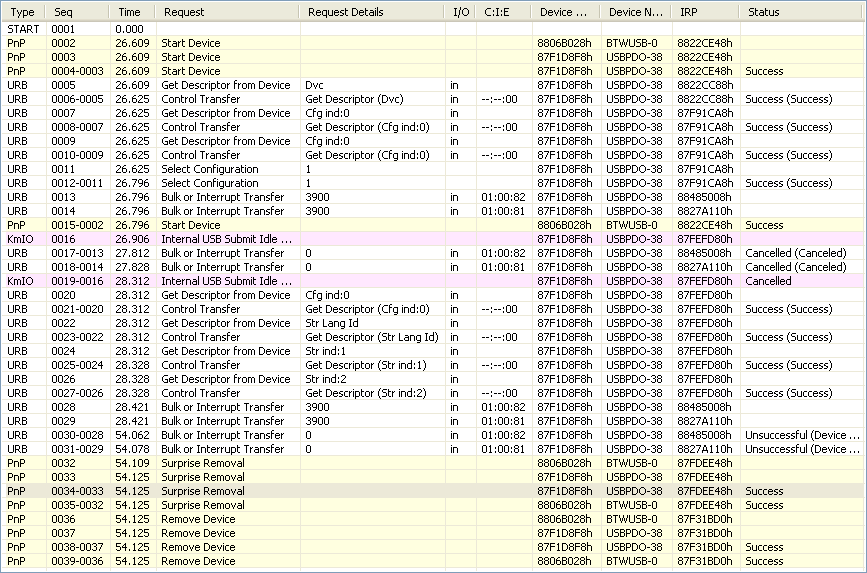
\includegraphics[width=\textwidth]{usblyzer}
\caption{Окно пакетов программы USBlyzer}
\label{usblyzer}
\end{figure}

\begin{figure}[h!]
\centering
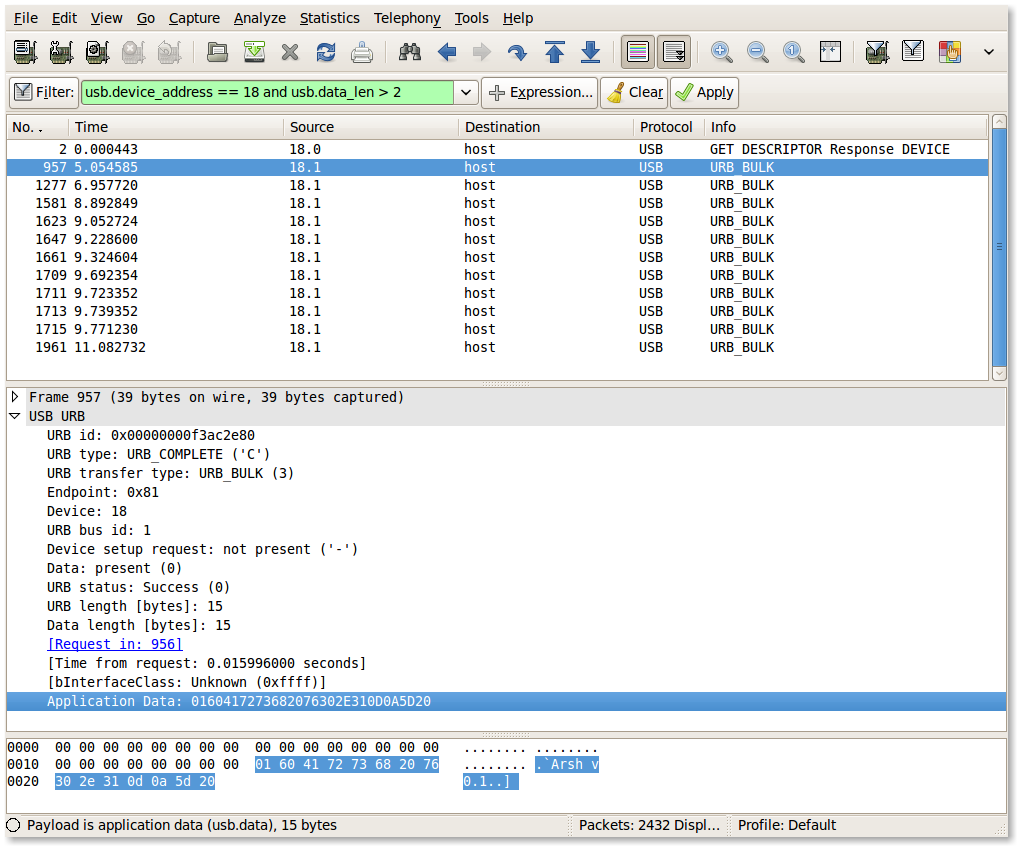
\includegraphics[width=\textwidth]{wireshark}
\caption{Окно пакетов программы Wireshark}
\label{wireshark}
\end{figure}

К сожалению, часть функционала устройства не удалось реализовать из-за ошибок в
самом устройстве, которые авторы сами обходили некими методами. Запрос насчёт
методов обхода этих ошибок не принёс результата. В частности, существует
проблема с работой режима отслеживания внезапных процессов.

\subsubsection{Подсистема USB}
Подсистема USB ядра Linux, \texttt{usbcore}, абстрагирует от разработчика
особенности конкретного компьютера и USB-контроллера и предоставляет
сравнительно удобный интерфейс для работы с USB. Основной единицей передачи
данных в подсистеме является URB-пакет --- специальная структура, заполняемая
при помощи процедур, предоставляемых подсистемой, которая содержит данные для
отправки на устройство или буфер для их получения и всю необходимую для этого
информацию. Подсистема также предоставляет автоматическое обнаружение
подключённых устройств. Работа с подсистемой выглядит так:
\begin{enumerate}
\item Разработчик создаёт статическую структуру \texttt{struct usb\_driver},
  заполняет её процедурами, которые будут вызываться из подсистемы при
  наступлении определённых событий. В заданных разработчиком процерурах должны
  быть процедуры \texttt{probe} и \texttt{release}, которые вызываются при
  нахождении устройства, похожего на управляемое данным драйвером, и при его
  отключании. Также разработчик создаёт и заполняет структуру \texttt{struct
    usb\_device\_id}, которая содержит идентификаторы управляемых драйвером
  устройств.
\item При обнаружении устройства вызывается процедура
  \texttt{probe}. Разработчик в ней должен проверить, совпадает ли устройство с
  тем которое контроллирует драйвер, занять память для своих данных, привязать
  их к устройству, обнаружить и сохранить в своих данных необходимые конечные
  точки и их параметры, а затем сообщить USB-подсистеме о готовности обслуживать
  устройство. Также разработчик может воспользоваться процедурами для создания
  привязанного к устройству символьного устройства, \texttt{usb\_register\_dev} и
  \texttt{usb\_unregister\_dev}. Для этого он также должен объявить структуры
  \texttt{struct usb\_class\_driver} и \texttt{struct file\_operations}, в которых
  будут также содержаться ссылки на функции, вызываемые при открытии
  пользователем соответствующего устройству файла или вызове конкретных операций
  над ним.
\item Драйвер далее волен работать самостоятельно, обычно обрабатывая обращения
  пользователя к файлу устройства.
\item При удалении устройства (которое может быть внезапным) вызывается
  процедура пользователя \texttt{release}, в которой он должен очистить память,
  прервать активные операции над устройством и вернуть ошибки.
\end{enumerate}
Также подсистема поддерживает усыпление и пробуждение устройств для сохранения
электроэнергии. Для того чтобы драйвер поддерживал это, разработчик должен
объявить методы \texttt{suspend}, \texttt{resume}, \texttt{pre\_reset},
\texttt{post\_reset} и установить параметр \texttt{.supports\_autosuspend}.

Для работы с URB-пакетами пользователь должен создать структуру \texttt{struct
  urb} с помощью \texttt{usb\_alloc\_urb} и заполнить её с помощью процедуры
\texttt{usb\_fill\_urb}, соответствующей типу нужной ему конечной точки. Также
пользователь должен занять память для буфера приёма или передачи. Буфер должен
обязательно находиться в куче, по возможности в памяти, которая используется для
DMA-операций с USB. Такой буфер создаётся при помощи процедуры
\texttt{usb\_alloc\_coherent}. Он обеспечивает более быструю работу с
USB-контроллером. Если такой буфер будет использоваться, то необходимо
установить флаг \texttt{URB\_NO\_TRANSFER\_DMA\_MAP} в поле
\texttt{.transfer\_flags} структуры \texttt{struct urb}. Также разработчик
назначает процедуру, которая будет вызвана по окончанию операции. После
окончания заполнения структуры, разработчик должен вызвать процедуру
\texttt{usb\_submit\_urb}, которая поместит операцию в очередь на выполнение.

Если пользователю необходимо контроллировать время и состояние операции, он
может воспользоваться так называемыми ``якорями''. Для этого ему нужно создать
структуру \texttt{struct usb\_anchor} и заполнить её процедурой
\texttt{init\_usb\_anchor}. После этого он может привязать операцию к якорю
процедурой \texttt{usb\_anchor\_urb}, что необходимо сделать до установки
URB-пакета в очередь на выполнение. После этого он может прервать выполнение
операции при помощи \texttt{usb\_kill\_anchored\_urbs} или подождать её
выполнения при помощи \texttt{usb\_wait\_anchor\_empty\_timeout}. Эта процедура
позволяет также задавать таймаут операции, что бывает полезно для обнаружения
слишком долгих передач.

В конце работы пользователь должен освободить память, занимаемую буфером, если
он был создан в DMA-дружественной памяти, при помощи
\texttt{usb\_free\_coherent}~\cite{usbskel}.

\subsubsection{Подсистема файловых устройств}
Эта подсистема используется чтобы создать псевдофайл, через который будет
выполняться взаимодействие с данным устройством. Существует много способов
создать такой файл и зарегистрировать его в подсистеме. Подсистема USB, в
частности, предоставляет свой, описанный выше способ.

После регистрации соответствующие процедуры начинают вызываться подсистемой при
вызове пользователем определённых системных вызовов над файлом. Кроме обычных
\texttt{open()}, \texttt{close()}, \texttt{read()} и \texttt{write()} существует
ещё много возможных определяемых вызовов. В частности, нас особенно интересует
вызов \texttt{ioctl()}, представленный в структуре \texttt{struct
  file\_operations} как \texttt{.unlocked\_ioctl}. Это связано с тем, что
начиная с версии ядра 2.6.11 разработчики улучшили механизмы занимания ресурсов
ядром, что позволило отказаться от части блокировок во время вызовов
\texttt{ioctl()}~\cite{newioctl}. Большинство определённых пользователем
процедур должны возвращать 0 или количество обработанных байт.

Особая ситуация обстоит с вызовом \texttt{llseek()}. Даже если разработчик не
хочет переопределять этот вызов, он всё равно будет доступен пользователю. Чтобы
не допустить использования пользователем этого вызова, следует в своём
обработчике \texttt{open()} вызвать процедуру \texttt{unseekable\_open()},
которая запретит этот вызов пользователю. Дополнительно следует установить поле
\texttt{.llseek} в структуре как \texttt{no\_llseek}.~\cite{corbet2009linux}.

\subsubsection{Блокировки в ядре Linux}
Библиотека блокировок ядра Linux содержит в себе крайне разнообразные
инструменты для обеспечения работы критических секций в коде. Мы рассмотрим
несколько инструментов:
\begin{itemize}
\item Спинлоки --- крайне быстрый метод взаимоблокировки, который сводится к
  введению ожидающего процессора в бесконечный цикл. Подобный метод
  взаимоблокировки может привести к входу процессора в бесконечный цикл, если
  спинлок используется в прерывании или в другом потоке на однопроцессорной
  машине, поэтому в таких случаях спинлок оптимизируется в пустую
  операцию. Однако, операции со спинлоками в ядре часто совмещены с операцией
  отключения прерываний, что само по себе обеспечивает блокировку на
  однопроцессорной системе. Поэтому если использовать спинлоки с отключением
  прерываний в обычном коде и простые спинлоки в коде прерываний, можно достичь
  очень быстрой работы. Спинлоки подходят для очень коротких критических секций,
  не более пары строк кода. Спинлоки инициализируются процедурой
  \texttt{spinlock\_init}, занятие и освобождение их выполняют процедуры
  \texttt{spin\_lock} и \texttt{spin\_unlock}, а отключающие прерывания версии ---
  \texttt{spin\_lock\_irqsave} и \texttt{spin\_unlock\_irqrestore}. Спинлоки не
  требуют освобождения памяти.
\item Мьютексы --- более продвинутый, но более медленный метод
  блокировки. Мьютексы позволяют переключать процессы, пока данный поток
  ждёт. Это обеспечивается за счёт более сложной архитектуры мьютексов, так что
  операции занятия на них достаточно трудоёмки. К тому же, мьютексы нельзя
  использовать в прерываниях. Однако они отлично подходят для синхронизации
  больших и потенциально долгих критических секций. Мьютексы инициализируются
  процедурой \texttt{mutex\_init}, занимаются и освобождаются процедурами
  \texttt{mutex\_lock} и \texttt{mutex\_unlock}, уничтожаются процедурой
  \texttt{mutex\_free}.
\item Завершения --- крайне удобный вариант блокировки для ожидания какого-либо
  события от другого потока. Завершения позволяют одному потоку ожидать
  (\texttt{wait\_completion}) события от другого потока (\texttt{complete} если
  требуется пробудить только один поток из очереди, или \texttt{complete\_all}
  если нужно пробудить все). Завершения инициализируются процедурой
  \texttt{init\_completion} и уничтожаются процедурой \texttt{free\_completion}.
\end{itemize}

\subsubsection{Использование потоков ядра}
Потоки ядра в ядре Linux проще в использовании чем \texttt{libpthread} или
похожие библиотеки потоков в режиме пользователя. Новый поток создаётся
процедурой \texttt{kthread\_create} или макросом \texttt{kthread\_run} который
сразу запускает созданный поток. Процедура потока должна после окончания
дождаться вызова \texttt{kthread\_should\_exit} со стороны создавшего потока,
для чего в конце можно создать бесконечный цикл. Со стороны создавшего потока
необходимо дождаться завершения работы процедурой \texttt{kthread\_exit}. В
модуле ядра поток используется после начальной инициализации для загрузки
прошивки в устройство и установки начальных параметров.

В драйвере защищены несколько величин:
\begin{itemize}
\item Текущее состояние (\texttt{enum state}) защищено спинлоком.
\item Операции ввода/вывода ограничены одной за раз мьютексом.
\item Текущие настройки осциллографа защищены спинлоком.
\end{itemize}

\subsubsection{Подсистема загрузки микропрограмм}
Эта подсистема избавляет разработчика от необходимости включать двоичный файл с
прошивкой устройства в модуль ядра, а также пытаться открыть и загрузить
прошивку из файловой системы, что крайне не приветствуется разработчиками ядра и
считается плохой практикой. Вместо этого, был добавлен метод
\texttt{request\_firmware}, которому как аргумент передаётся название необходимой
микропрограммы. Ядро запрашивает у демона устройств режима пользователя
(\texttt{udev}) о наличии такого файла, и при наличии, демон загружает файл в
ядро. Затем функция возвращает управление модулю, возвращая структуру
\texttt{struct firmware}, в которой и находится загруженный файл. После
окончания работы структуру необходимо освободить процедурой
\texttt{free\_firmware}.

\subsubsection{Подсчёт ссылок}
Ядро Linux содержит также механизм \texttt{kref} для подсчёта ссылок и
автоматического уничтожения структур данных в памяти. Для этого отслеживаемая
структура должна содержать поле типа \texttt{struct kref}, которое
инициализируется (с числом ссылок 1) методом \texttt{kref\_init}. Затем
количество ссылок увеличивается процедурой \texttt{kref\_get} и уменьшается
процедурой \texttt{kref\_put}. При достижении нулевого числа ссылок вызывается
пользовательский метод, которому передаётся указатель на структуру и который
отвечает за правильное уничтожение структуры.

\subsubsection{Триггер и чтение}
Вызов триггера в драйвере --- единственная асинхронная операция, доступная
пользователю. Триггер после подтверждения чтения данных с осциллографа начинает
чтение данных с него. Если в это время вызывается метод \texttt{read()}, он
блокирует пользовательскую программу до конца передачи данных. Схемы алгоритмов
представлены в виде блок-схем на рисунках~\ref{algo1} и~\ref{algo2}.

\begin{figure}[h!]
\centering
% Graphic for TeX using PGF
% Title: /home/abbradar/scope/doc/algo1.dia
% Creator: Dia v0.97.2
% CreationDate: Mon May 27 16:02:47 2013
% For: abbradar
% \usepackage{tikz}
% The following commands are not supported in PSTricks at present
% We define them conditionally, so when they are implemented,
% this pgf file will use them.
\ifx\du\undefined
  \newlength{\du}
\fi
\setlength{\du}{15\unitlength}
\begin{tikzpicture}
\pgftransformxscale{1.000000}
\pgftransformyscale{-1.000000}
\definecolor{dialinecolor}{rgb}{0.000000, 0.000000, 0.000000}
\pgfsetstrokecolor{dialinecolor}
\definecolor{dialinecolor}{rgb}{1.000000, 1.000000, 1.000000}
\pgfsetfillcolor{dialinecolor}
\pgfsetlinewidth{0.100000\du}
\pgfsetdash{}{0pt}
\pgfsetdash{}{0pt}
\pgfsetbuttcap
\pgfsetmiterjoin
\pgfsetlinewidth{0.100000\du}
\pgfsetbuttcap
\pgfsetmiterjoin
\pgfsetdash{}{0pt}
\definecolor{dialinecolor}{rgb}{1.000000, 1.000000, 1.000000}
\pgfsetfillcolor{dialinecolor}
\pgfpathmoveto{\pgfpoint{12.500000\du}{1.000000\du}}
\pgfpathlineto{\pgfpoint{18.500000\du}{1.000000\du}}
\pgfpathcurveto{\pgfpoint{19.328428\du}{1.000000\du}}{\pgfpoint{20.000000\du}{1.671572\du}}{\pgfpoint{20.000000\du}{2.500000\du}}
\pgfpathcurveto{\pgfpoint{20.000000\du}{3.328428\du}}{\pgfpoint{19.328428\du}{4.000000\du}}{\pgfpoint{18.500000\du}{4.000000\du}}
\pgfpathlineto{\pgfpoint{12.500000\du}{4.000000\du}}
\pgfpathcurveto{\pgfpoint{11.671572\du}{4.000000\du}}{\pgfpoint{11.000000\du}{3.328428\du}}{\pgfpoint{11.000000\du}{2.500000\du}}
\pgfpathcurveto{\pgfpoint{11.000000\du}{1.671573\du}}{\pgfpoint{11.671572\du}{1.000000\du}}{\pgfpoint{12.500000\du}{1.000000\du}}
\pgfusepath{fill}
\definecolor{dialinecolor}{rgb}{0.000000, 0.000000, 0.000000}
\pgfsetstrokecolor{dialinecolor}
\pgfpathmoveto{\pgfpoint{12.500000\du}{1.000000\du}}
\pgfpathlineto{\pgfpoint{18.500000\du}{1.000000\du}}
\pgfpathcurveto{\pgfpoint{19.328428\du}{1.000000\du}}{\pgfpoint{20.000000\du}{1.671572\du}}{\pgfpoint{20.000000\du}{2.500000\du}}
\pgfpathcurveto{\pgfpoint{20.000000\du}{3.328428\du}}{\pgfpoint{19.328428\du}{4.000000\du}}{\pgfpoint{18.500000\du}{4.000000\du}}
\pgfpathlineto{\pgfpoint{12.500000\du}{4.000000\du}}
\pgfpathcurveto{\pgfpoint{11.671572\du}{4.000000\du}}{\pgfpoint{11.000000\du}{3.328428\du}}{\pgfpoint{11.000000\du}{2.500000\du}}
\pgfpathcurveto{\pgfpoint{11.000000\du}{1.671573\du}}{\pgfpoint{11.671572\du}{1.000000\du}}{\pgfpoint{12.500000\du}{1.000000\du}}
\pgfusepath{stroke}
% setfont left to latex
\definecolor{dialinecolor}{rgb}{0.000000, 0.000000, 0.000000}
\pgfsetstrokecolor{dialinecolor}
\node at (15.500000\du,2.700000\du){Начало};
\definecolor{dialinecolor}{rgb}{1.000000, 1.000000, 1.000000}
\pgfsetfillcolor{dialinecolor}
\fill (11.000000\du,6.000000\du)--(11.000000\du,8.700000\du)--(20.000000\du,8.700000\du)--(20.000000\du,6.000000\du)--cycle;
\pgfsetlinewidth{0.100000\du}
\pgfsetdash{}{0pt}
\pgfsetdash{}{0pt}
\pgfsetmiterjoin
\definecolor{dialinecolor}{rgb}{0.000000, 0.000000, 0.000000}
\pgfsetstrokecolor{dialinecolor}
\draw (11.000000\du,6.000000\du)--(11.000000\du,8.700000\du)--(20.000000\du,8.700000\du)--(20.000000\du,6.000000\du)--cycle;
% setfont left to latex
\definecolor{dialinecolor}{rgb}{0.000000, 0.000000, 0.000000}
\pgfsetstrokecolor{dialinecolor}
\node at (15.500000\du,7.130000\du){Отправить команду};
% setfont left to latex
\definecolor{dialinecolor}{rgb}{0.000000, 0.000000, 0.000000}
\pgfsetstrokecolor{dialinecolor}
\node at (15.500000\du,7.930000\du){триггера};
\pgfsetlinewidth{0.100000\du}
\pgfsetdash{}{0pt}
\pgfsetdash{}{0pt}
\pgfsetbuttcap
{
\definecolor{dialinecolor}{rgb}{0.000000, 0.000000, 0.000000}
\pgfsetfillcolor{dialinecolor}
% was here!!!
\pgfsetarrowsend{stealth}
\definecolor{dialinecolor}{rgb}{0.000000, 0.000000, 0.000000}
\pgfsetstrokecolor{dialinecolor}
\draw (15.500000\du,4.000000\du)--(15.500000\du,6.000000\du);
}
\pgfsetlinewidth{0.100000\du}
\pgfsetdash{}{0pt}
\pgfsetdash{}{0pt}
\pgfsetbuttcap
{
\definecolor{dialinecolor}{rgb}{0.000000, 0.000000, 0.000000}
\pgfsetfillcolor{dialinecolor}
% was here!!!
\pgfsetarrowsend{stealth}
\definecolor{dialinecolor}{rgb}{0.000000, 0.000000, 0.000000}
\pgfsetstrokecolor{dialinecolor}
\draw (15.500000\du,8.700000\du)--(15.500000\du,11.000000\du);
}
% setfont left to latex
\definecolor{dialinecolor}{rgb}{0.000000, 0.000000, 0.000000}
\pgfsetstrokecolor{dialinecolor}
\node[anchor=west] at (21.000000\du,13.000000\du){нет};
% setfont left to latex
\definecolor{dialinecolor}{rgb}{0.000000, 0.000000, 0.000000}
\pgfsetstrokecolor{dialinecolor}
\node[anchor=west] at (15.600100\du,15.600000\du){};
% setfont left to latex
\definecolor{dialinecolor}{rgb}{0.000000, 0.000000, 0.000000}
\pgfsetstrokecolor{dialinecolor}
\node[anchor=west] at (14.000000\du,17.000000\du){да};
\definecolor{dialinecolor}{rgb}{1.000000, 1.000000, 1.000000}
\pgfsetfillcolor{dialinecolor}
\fill (11.000000\du,19.000000\du)--(11.000000\du,22.000000\du)--(20.000000\du,22.000000\du)--(20.000000\du,19.000000\du)--cycle;
\pgfsetlinewidth{0.100000\du}
\pgfsetdash{}{0pt}
\pgfsetdash{}{0pt}
\pgfsetmiterjoin
\definecolor{dialinecolor}{rgb}{0.000000, 0.000000, 0.000000}
\pgfsetstrokecolor{dialinecolor}
\draw (11.000000\du,19.000000\du)--(11.000000\du,22.000000\du)--(20.000000\du,22.000000\du)--(20.000000\du,19.000000\du)--cycle;
% setfont left to latex
\definecolor{dialinecolor}{rgb}{0.000000, 0.000000, 0.000000}
\pgfsetstrokecolor{dialinecolor}
\node at (15.500000\du,20.280000\du){Считать символ от};
% setfont left to latex
\definecolor{dialinecolor}{rgb}{0.000000, 0.000000, 0.000000}
\pgfsetstrokecolor{dialinecolor}
\node at (15.500000\du,21.080000\du){устройства};
\definecolor{dialinecolor}{rgb}{1.000000, 1.000000, 1.000000}
\pgfsetfillcolor{dialinecolor}
\fill (15.500000\du,11.000000\du)--(20.000000\du,13.500000\du)--(15.500000\du,16.000000\du)--(11.000000\du,13.500000\du)--cycle;
\pgfsetlinewidth{0.100000\du}
\pgfsetdash{}{0pt}
\pgfsetdash{}{0pt}
\pgfsetmiterjoin
\definecolor{dialinecolor}{rgb}{0.000000, 0.000000, 0.000000}
\pgfsetstrokecolor{dialinecolor}
\draw (15.500000\du,11.000000\du)--(20.000000\du,13.500000\du)--(15.500000\du,16.000000\du)--(11.000000\du,13.500000\du)--cycle;
% setfont left to latex
\definecolor{dialinecolor}{rgb}{0.000000, 0.000000, 0.000000}
\pgfsetstrokecolor{dialinecolor}
\node at (15.500000\du,13.280000\du){Произошла};
% setfont left to latex
\definecolor{dialinecolor}{rgb}{0.000000, 0.000000, 0.000000}
\pgfsetstrokecolor{dialinecolor}
\node at (15.500000\du,14.080000\du){ошибка?};
\pgfsetlinewidth{0.100000\du}
\pgfsetdash{}{0pt}
\pgfsetdash{}{0pt}
\pgfsetbuttcap
{
\definecolor{dialinecolor}{rgb}{0.000000, 0.000000, 0.000000}
\pgfsetfillcolor{dialinecolor}
% was here!!!
\pgfsetarrowsend{stealth}
\definecolor{dialinecolor}{rgb}{0.000000, 0.000000, 0.000000}
\pgfsetstrokecolor{dialinecolor}
\draw (15.500000\du,16.000000\du)--(15.500000\du,18.950378\du);
}
\definecolor{dialinecolor}{rgb}{1.000000, 1.000000, 1.000000}
\pgfsetfillcolor{dialinecolor}
\fill (15.500000\du,24.000000\du)--(20.000000\du,26.500000\du)--(15.500000\du,29.000000\du)--(11.000000\du,26.500000\du)--cycle;
\pgfsetlinewidth{0.100000\du}
\pgfsetdash{}{0pt}
\pgfsetdash{}{0pt}
\pgfsetmiterjoin
\definecolor{dialinecolor}{rgb}{0.000000, 0.000000, 0.000000}
\pgfsetstrokecolor{dialinecolor}
\draw (15.500000\du,24.000000\du)--(20.000000\du,26.500000\du)--(15.500000\du,29.000000\du)--(11.000000\du,26.500000\du)--cycle;
% setfont left to latex
\definecolor{dialinecolor}{rgb}{0.000000, 0.000000, 0.000000}
\pgfsetstrokecolor{dialinecolor}
\node at (15.500000\du,26.280000\du){Триггер};
% setfont left to latex
\definecolor{dialinecolor}{rgb}{0.000000, 0.000000, 0.000000}
\pgfsetstrokecolor{dialinecolor}
\node at (15.500000\du,27.080000\du){сработал?};
\pgfsetlinewidth{0.100000\du}
\pgfsetdash{}{0pt}
\pgfsetdash{}{0pt}
\pgfsetbuttcap
{
\definecolor{dialinecolor}{rgb}{0.000000, 0.000000, 0.000000}
\pgfsetfillcolor{dialinecolor}
% was here!!!
\pgfsetarrowsend{stealth}
\definecolor{dialinecolor}{rgb}{0.000000, 0.000000, 0.000000}
\pgfsetstrokecolor{dialinecolor}
\draw (15.500000\du,22.000000\du)--(15.500000\du,24.000000\du);
}
\pgfsetlinewidth{0.100000\du}
\pgfsetdash{}{0pt}
\pgfsetdash{}{0pt}
\pgfsetmiterjoin
\pgfsetbuttcap
{
\definecolor{dialinecolor}{rgb}{0.000000, 0.000000, 0.000000}
\pgfsetfillcolor{dialinecolor}
% was here!!!
\pgfsetarrowsend{stealth}
{\pgfsetcornersarced{\pgfpoint{0.000000\du}{0.000000\du}}\definecolor{dialinecolor}{rgb}{0.000000, 0.000000, 0.000000}
\pgfsetstrokecolor{dialinecolor}
\draw (20.000000\du,26.500000\du)--(23.000000\du,26.500000\du)--(23.000000\du,17.475189\du)--(15.500000\du,17.475189\du);
}}
% setfont left to latex
\definecolor{dialinecolor}{rgb}{0.000000, 0.000000, 0.000000}
\pgfsetstrokecolor{dialinecolor}
\node[anchor=west] at (21.000000\du,26.000000\du){нет};
\definecolor{dialinecolor}{rgb}{1.000000, 1.000000, 1.000000}
\pgfsetfillcolor{dialinecolor}
\fill (11.000000\du,32.000000\du)--(11.000000\du,35.000000\du)--(20.000000\du,35.000000\du)--(20.000000\du,32.000000\du)--cycle;
\pgfsetlinewidth{0.100000\du}
\pgfsetdash{}{0pt}
\pgfsetdash{}{0pt}
\pgfsetmiterjoin
\definecolor{dialinecolor}{rgb}{0.000000, 0.000000, 0.000000}
\pgfsetstrokecolor{dialinecolor}
\draw (11.000000\du,32.000000\du)--(11.000000\du,35.000000\du)--(20.000000\du,35.000000\du)--(20.000000\du,32.000000\du)--cycle;
% setfont left to latex
\definecolor{dialinecolor}{rgb}{0.000000, 0.000000, 0.000000}
\pgfsetstrokecolor{dialinecolor}
\node at (15.500000\du,33.680000\du){Начать приём данных};
\pgfsetlinewidth{0.100000\du}
\pgfsetdash{}{0pt}
\pgfsetdash{}{0pt}
\pgfsetbuttcap
{
\definecolor{dialinecolor}{rgb}{0.000000, 0.000000, 0.000000}
\pgfsetfillcolor{dialinecolor}
% was here!!!
\pgfsetarrowsend{stealth}
\definecolor{dialinecolor}{rgb}{0.000000, 0.000000, 0.000000}
\pgfsetstrokecolor{dialinecolor}
\draw (15.500000\du,29.000000\du)--(15.500000\du,32.000000\du);
}
% setfont left to latex
\definecolor{dialinecolor}{rgb}{0.000000, 0.000000, 0.000000}
\pgfsetstrokecolor{dialinecolor}
\node[anchor=west] at (16.000000\du,30.000000\du){};
% setfont left to latex
\definecolor{dialinecolor}{rgb}{0.000000, 0.000000, 0.000000}
\pgfsetstrokecolor{dialinecolor}
\node[anchor=west] at (16.000000\du,30.000000\du){да};
\pgfsetlinewidth{0.100000\du}
\pgfsetdash{}{0pt}
\pgfsetdash{}{0pt}
\pgfsetbuttcap
\pgfsetmiterjoin
\pgfsetlinewidth{0.100000\du}
\pgfsetbuttcap
\pgfsetmiterjoin
\pgfsetdash{}{0pt}
\definecolor{dialinecolor}{rgb}{1.000000, 1.000000, 1.000000}
\pgfsetfillcolor{dialinecolor}
\pgfpathmoveto{\pgfpoint{12.500000\du}{38.000000\du}}
\pgfpathlineto{\pgfpoint{18.500000\du}{38.000000\du}}
\pgfpathcurveto{\pgfpoint{19.328428\du}{38.000000\du}}{\pgfpoint{20.000000\du}{38.671572\du}}{\pgfpoint{20.000000\du}{39.500000\du}}
\pgfpathcurveto{\pgfpoint{20.000000\du}{40.328428\du}}{\pgfpoint{19.328428\du}{41.000000\du}}{\pgfpoint{18.500000\du}{41.000000\du}}
\pgfpathlineto{\pgfpoint{12.500000\du}{41.000000\du}}
\pgfpathcurveto{\pgfpoint{11.671572\du}{41.000000\du}}{\pgfpoint{11.000000\du}{40.328428\du}}{\pgfpoint{11.000000\du}{39.500000\du}}
\pgfpathcurveto{\pgfpoint{11.000000\du}{38.671573\du}}{\pgfpoint{11.671572\du}{38.000000\du}}{\pgfpoint{12.500000\du}{38.000000\du}}
\pgfusepath{fill}
\definecolor{dialinecolor}{rgb}{0.000000, 0.000000, 0.000000}
\pgfsetstrokecolor{dialinecolor}
\pgfpathmoveto{\pgfpoint{12.500000\du}{38.000000\du}}
\pgfpathlineto{\pgfpoint{18.500000\du}{38.000000\du}}
\pgfpathcurveto{\pgfpoint{19.328428\du}{38.000000\du}}{\pgfpoint{20.000000\du}{38.671572\du}}{\pgfpoint{20.000000\du}{39.500000\du}}
\pgfpathcurveto{\pgfpoint{20.000000\du}{40.328428\du}}{\pgfpoint{19.328428\du}{41.000000\du}}{\pgfpoint{18.500000\du}{41.000000\du}}
\pgfpathlineto{\pgfpoint{12.500000\du}{41.000000\du}}
\pgfpathcurveto{\pgfpoint{11.671572\du}{41.000000\du}}{\pgfpoint{11.000000\du}{40.328428\du}}{\pgfpoint{11.000000\du}{39.500000\du}}
\pgfpathcurveto{\pgfpoint{11.000000\du}{38.671573\du}}{\pgfpoint{11.671572\du}{38.000000\du}}{\pgfpoint{12.500000\du}{38.000000\du}}
\pgfusepath{stroke}
% setfont left to latex
\definecolor{dialinecolor}{rgb}{0.000000, 0.000000, 0.000000}
\pgfsetstrokecolor{dialinecolor}
\node at (15.500000\du,39.700000\du){Конец};
\pgfsetlinewidth{0.100000\du}
\pgfsetdash{}{0pt}
\pgfsetdash{}{0pt}
\pgfsetbuttcap
{
\definecolor{dialinecolor}{rgb}{0.000000, 0.000000, 0.000000}
\pgfsetfillcolor{dialinecolor}
% was here!!!
\pgfsetarrowsend{stealth}
\definecolor{dialinecolor}{rgb}{0.000000, 0.000000, 0.000000}
\pgfsetstrokecolor{dialinecolor}
\draw (15.500000\du,35.049622\du)--(15.500000\du,38.000000\du);
}
% setfont left to latex
\definecolor{dialinecolor}{rgb}{0.000000, 0.000000, 0.000000}
\pgfsetstrokecolor{dialinecolor}
\node[anchor=west] at (16.000000\du,36.000000\du){};
\definecolor{dialinecolor}{rgb}{1.000000, 1.000000, 1.000000}
\pgfsetfillcolor{dialinecolor}
\fill (24.000000\du,19.000000\du)--(24.000000\du,22.000000\du)--(32.000000\du,22.000000\du)--(32.000000\du,19.000000\du)--cycle;
\pgfsetlinewidth{0.100000\du}
\pgfsetdash{}{0pt}
\pgfsetdash{}{0pt}
\pgfsetmiterjoin
\definecolor{dialinecolor}{rgb}{0.000000, 0.000000, 0.000000}
\pgfsetstrokecolor{dialinecolor}
\draw (24.000000\du,19.000000\du)--(24.000000\du,22.000000\du)--(32.000000\du,22.000000\du)--(32.000000\du,19.000000\du)--cycle;
% setfont left to latex
\definecolor{dialinecolor}{rgb}{0.000000, 0.000000, 0.000000}
\pgfsetstrokecolor{dialinecolor}
\node at (28.000000\du,20.680000\du){Обработка ошибки};
\pgfsetlinewidth{0.100000\du}
\pgfsetdash{}{0pt}
\pgfsetdash{}{0pt}
\pgfsetmiterjoin
\pgfsetbuttcap
{
\definecolor{dialinecolor}{rgb}{0.000000, 0.000000, 0.000000}
\pgfsetfillcolor{dialinecolor}
% was here!!!
\pgfsetarrowsend{stealth}
{\pgfsetcornersarced{\pgfpoint{0.000000\du}{0.000000\du}}\definecolor{dialinecolor}{rgb}{0.000000, 0.000000, 0.000000}
\pgfsetstrokecolor{dialinecolor}
\draw (28.000000\du,22.000000\du)--(28.000000\du,36.524811\du)--(15.500000\du,36.524811\du);
}}
\pgfsetlinewidth{0.100000\du}
\pgfsetdash{}{0pt}
\pgfsetdash{}{0pt}
\pgfsetmiterjoin
\pgfsetbuttcap
{
\definecolor{dialinecolor}{rgb}{0.000000, 0.000000, 0.000000}
\pgfsetfillcolor{dialinecolor}
% was here!!!
\pgfsetarrowsend{stealth}
{\pgfsetcornersarced{\pgfpoint{0.000000\du}{0.000000\du}}\definecolor{dialinecolor}{rgb}{0.000000, 0.000000, 0.000000}
\pgfsetstrokecolor{dialinecolor}
\draw (20.000000\du,13.500000\du)--(20.000000\du,13.562500\du)--(28.000000\du,13.562500\du)--(28.000000\du,19.000000\du);
}}
\end{tikzpicture}

\label{algo1}
\caption{Алгоритм процедуры триггера}
\end{figure}

\begin{figure}[h!]
\centering
% Graphic for TeX using PGF
% Title: /home/abbradar/scope/doc/algo2.dia
% Creator: Dia v0.97.2
% CreationDate: Mon May 27 16:00:40 2013
% For: abbradar
% \usepackage{tikz}
% The following commands are not supported in PSTricks at present
% We define them conditionally, so when they are implemented,
% this pgf file will use them.
\ifx\du\undefined
  \newlength{\du}
\fi
\setlength{\du}{15\unitlength}
\begin{tikzpicture}
\pgftransformxscale{1.000000}
\pgftransformyscale{-1.000000}
\definecolor{dialinecolor}{rgb}{0.000000, 0.000000, 0.000000}
\pgfsetstrokecolor{dialinecolor}
\definecolor{dialinecolor}{rgb}{1.000000, 1.000000, 1.000000}
\pgfsetfillcolor{dialinecolor}
\pgfsetlinewidth{0.100000\du}
\pgfsetdash{}{0pt}
\pgfsetdash{}{0pt}
\pgfsetbuttcap
\pgfsetmiterjoin
\pgfsetlinewidth{0.100000\du}
\pgfsetbuttcap
\pgfsetmiterjoin
\pgfsetdash{}{0pt}
\definecolor{dialinecolor}{rgb}{1.000000, 1.000000, 1.000000}
\pgfsetfillcolor{dialinecolor}
\pgfpathmoveto{\pgfpoint{9.500000\du}{2.000000\du}}
\pgfpathlineto{\pgfpoint{15.500000\du}{2.000000\du}}
\pgfpathcurveto{\pgfpoint{16.328428\du}{2.000000\du}}{\pgfpoint{17.000000\du}{2.671572\du}}{\pgfpoint{17.000000\du}{3.500000\du}}
\pgfpathcurveto{\pgfpoint{17.000000\du}{4.328427\du}}{\pgfpoint{16.328428\du}{5.000000\du}}{\pgfpoint{15.500000\du}{5.000000\du}}
\pgfpathlineto{\pgfpoint{9.500000\du}{5.000000\du}}
\pgfpathcurveto{\pgfpoint{8.671572\du}{5.000000\du}}{\pgfpoint{8.000000\du}{4.328427\du}}{\pgfpoint{8.000000\du}{3.500000\du}}
\pgfpathcurveto{\pgfpoint{8.000000\du}{2.671572\du}}{\pgfpoint{8.671572\du}{2.000000\du}}{\pgfpoint{9.500000\du}{2.000000\du}}
\pgfusepath{fill}
\definecolor{dialinecolor}{rgb}{0.000000, 0.000000, 0.000000}
\pgfsetstrokecolor{dialinecolor}
\pgfpathmoveto{\pgfpoint{9.500000\du}{2.000000\du}}
\pgfpathlineto{\pgfpoint{15.500000\du}{2.000000\du}}
\pgfpathcurveto{\pgfpoint{16.328428\du}{2.000000\du}}{\pgfpoint{17.000000\du}{2.671572\du}}{\pgfpoint{17.000000\du}{3.500000\du}}
\pgfpathcurveto{\pgfpoint{17.000000\du}{4.328427\du}}{\pgfpoint{16.328428\du}{5.000000\du}}{\pgfpoint{15.500000\du}{5.000000\du}}
\pgfpathlineto{\pgfpoint{9.500000\du}{5.000000\du}}
\pgfpathcurveto{\pgfpoint{8.671572\du}{5.000000\du}}{\pgfpoint{8.000000\du}{4.328427\du}}{\pgfpoint{8.000000\du}{3.500000\du}}
\pgfpathcurveto{\pgfpoint{8.000000\du}{2.671572\du}}{\pgfpoint{8.671572\du}{2.000000\du}}{\pgfpoint{9.500000\du}{2.000000\du}}
\pgfusepath{stroke}
% setfont left to latex
\definecolor{dialinecolor}{rgb}{0.000000, 0.000000, 0.000000}
\pgfsetstrokecolor{dialinecolor}
\node at (12.500000\du,3.700000\du){Начало};
\pgfsetlinewidth{0.100000\du}
\pgfsetdash{}{0pt}
\pgfsetdash{}{0pt}
\pgfsetbuttcap
{
\definecolor{dialinecolor}{rgb}{0.000000, 0.000000, 0.000000}
\pgfsetfillcolor{dialinecolor}
% was here!!!
\pgfsetarrowsend{stealth}
\definecolor{dialinecolor}{rgb}{0.000000, 0.000000, 0.000000}
\pgfsetstrokecolor{dialinecolor}
\draw (12.500000\du,5.000000\du)--(12.500000\du,7.000000\du);
}
% setfont left to latex
\definecolor{dialinecolor}{rgb}{0.000000, 0.000000, 0.000000}
\pgfsetstrokecolor{dialinecolor}
\node[anchor=west] at (13.000000\du,14.000000\du){да};
% setfont left to latex
\definecolor{dialinecolor}{rgb}{0.000000, 0.000000, 0.000000}
\pgfsetstrokecolor{dialinecolor}
\node[anchor=west] at (12.600100\du,16.600000\du){};
\definecolor{dialinecolor}{rgb}{1.000000, 1.000000, 1.000000}
\pgfsetfillcolor{dialinecolor}
\fill (8.000000\du,25.000000\du)--(8.000000\du,27.700000\du)--(17.000000\du,27.700000\du)--(17.000000\du,25.000000\du)--cycle;
\pgfsetlinewidth{0.100000\du}
\pgfsetdash{}{0pt}
\pgfsetdash{}{0pt}
\pgfsetmiterjoin
\definecolor{dialinecolor}{rgb}{0.000000, 0.000000, 0.000000}
\pgfsetstrokecolor{dialinecolor}
\draw (8.000000\du,25.000000\du)--(8.000000\du,27.700000\du)--(17.000000\du,27.700000\du)--(17.000000\du,25.000000\du)--cycle;
% setfont left to latex
\definecolor{dialinecolor}{rgb}{0.000000, 0.000000, 0.000000}
\pgfsetstrokecolor{dialinecolor}
\node at (12.500000\du,26.130000\du){Скопировать};
% setfont left to latex
\definecolor{dialinecolor}{rgb}{0.000000, 0.000000, 0.000000}
\pgfsetstrokecolor{dialinecolor}
\node at (12.500000\du,26.930000\du){данные в буфер};
\definecolor{dialinecolor}{rgb}{1.000000, 1.000000, 1.000000}
\pgfsetfillcolor{dialinecolor}
\fill (12.500000\du,7.000000\du)--(17.000000\du,9.500000\du)--(12.500000\du,12.000000\du)--(8.000000\du,9.500000\du)--cycle;
\pgfsetlinewidth{0.100000\du}
\pgfsetdash{}{0pt}
\pgfsetdash{}{0pt}
\pgfsetmiterjoin
\definecolor{dialinecolor}{rgb}{0.000000, 0.000000, 0.000000}
\pgfsetstrokecolor{dialinecolor}
\draw (12.500000\du,7.000000\du)--(17.000000\du,9.500000\du)--(12.500000\du,12.000000\du)--(8.000000\du,9.500000\du)--cycle;
% setfont left to latex
\definecolor{dialinecolor}{rgb}{0.000000, 0.000000, 0.000000}
\pgfsetstrokecolor{dialinecolor}
\node at (12.500000\du,9.680000\du){Данные готовы?};
\pgfsetlinewidth{0.100000\du}
\pgfsetdash{}{0pt}
\pgfsetdash{}{0pt}
\pgfsetbuttcap
{
\definecolor{dialinecolor}{rgb}{0.000000, 0.000000, 0.000000}
\pgfsetfillcolor{dialinecolor}
% was here!!!
\pgfsetarrowsend{stealth}
\definecolor{dialinecolor}{rgb}{0.000000, 0.000000, 0.000000}
\pgfsetstrokecolor{dialinecolor}
\draw (12.500000\du,12.000000\du)--(12.500000\du,24.949947\du);
}
\definecolor{dialinecolor}{rgb}{1.000000, 1.000000, 1.000000}
\pgfsetfillcolor{dialinecolor}
\fill (8.000000\du,30.000000\du)--(8.000000\du,33.000000\du)--(17.000000\du,33.000000\du)--(17.000000\du,30.000000\du)--cycle;
\pgfsetlinewidth{0.100000\du}
\pgfsetdash{}{0pt}
\pgfsetdash{}{0pt}
\pgfsetmiterjoin
\definecolor{dialinecolor}{rgb}{0.000000, 0.000000, 0.000000}
\pgfsetstrokecolor{dialinecolor}
\draw (8.000000\du,30.000000\du)--(8.000000\du,33.000000\du)--(17.000000\du,33.000000\du)--(17.000000\du,30.000000\du)--cycle;
% setfont left to latex
\definecolor{dialinecolor}{rgb}{0.000000, 0.000000, 0.000000}
\pgfsetstrokecolor{dialinecolor}
\node at (12.500000\du,31.280000\du){Уменьшить счётчик};
% setfont left to latex
\definecolor{dialinecolor}{rgb}{0.000000, 0.000000, 0.000000}
\pgfsetstrokecolor{dialinecolor}
\node at (12.500000\du,32.080000\du){доступных данных};
% setfont left to latex
\definecolor{dialinecolor}{rgb}{0.000000, 0.000000, 0.000000}
\pgfsetstrokecolor{dialinecolor}
\node[anchor=west] at (13.000000\du,31.000000\du){};
\pgfsetlinewidth{0.100000\du}
\pgfsetdash{}{0pt}
\pgfsetdash{}{0pt}
\pgfsetbuttcap
\pgfsetmiterjoin
\pgfsetlinewidth{0.100000\du}
\pgfsetbuttcap
\pgfsetmiterjoin
\pgfsetdash{}{0pt}
\definecolor{dialinecolor}{rgb}{1.000000, 1.000000, 1.000000}
\pgfsetfillcolor{dialinecolor}
\pgfpathmoveto{\pgfpoint{9.500000\du}{36.000000\du}}
\pgfpathlineto{\pgfpoint{15.500000\du}{36.000000\du}}
\pgfpathcurveto{\pgfpoint{16.328428\du}{36.000000\du}}{\pgfpoint{17.000000\du}{36.671572\du}}{\pgfpoint{17.000000\du}{37.500000\du}}
\pgfpathcurveto{\pgfpoint{17.000000\du}{38.328428\du}}{\pgfpoint{16.328428\du}{39.000000\du}}{\pgfpoint{15.500000\du}{39.000000\du}}
\pgfpathlineto{\pgfpoint{9.500000\du}{39.000000\du}}
\pgfpathcurveto{\pgfpoint{8.671572\du}{39.000000\du}}{\pgfpoint{8.000000\du}{38.328428\du}}{\pgfpoint{8.000000\du}{37.500000\du}}
\pgfpathcurveto{\pgfpoint{8.000000\du}{36.671573\du}}{\pgfpoint{8.671572\du}{36.000000\du}}{\pgfpoint{9.500000\du}{36.000000\du}}
\pgfusepath{fill}
\definecolor{dialinecolor}{rgb}{0.000000, 0.000000, 0.000000}
\pgfsetstrokecolor{dialinecolor}
\pgfpathmoveto{\pgfpoint{9.500000\du}{36.000000\du}}
\pgfpathlineto{\pgfpoint{15.500000\du}{36.000000\du}}
\pgfpathcurveto{\pgfpoint{16.328428\du}{36.000000\du}}{\pgfpoint{17.000000\du}{36.671572\du}}{\pgfpoint{17.000000\du}{37.500000\du}}
\pgfpathcurveto{\pgfpoint{17.000000\du}{38.328428\du}}{\pgfpoint{16.328428\du}{39.000000\du}}{\pgfpoint{15.500000\du}{39.000000\du}}
\pgfpathlineto{\pgfpoint{9.500000\du}{39.000000\du}}
\pgfpathcurveto{\pgfpoint{8.671572\du}{39.000000\du}}{\pgfpoint{8.000000\du}{38.328428\du}}{\pgfpoint{8.000000\du}{37.500000\du}}
\pgfpathcurveto{\pgfpoint{8.000000\du}{36.671573\du}}{\pgfpoint{8.671572\du}{36.000000\du}}{\pgfpoint{9.500000\du}{36.000000\du}}
\pgfusepath{stroke}
% setfont left to latex
\definecolor{dialinecolor}{rgb}{0.000000, 0.000000, 0.000000}
\pgfsetstrokecolor{dialinecolor}
\node at (12.500000\du,37.700000\du){Конец};
\pgfsetlinewidth{0.100000\du}
\pgfsetdash{}{0pt}
\pgfsetdash{}{0pt}
\pgfsetbuttcap
{
\definecolor{dialinecolor}{rgb}{0.000000, 0.000000, 0.000000}
\pgfsetfillcolor{dialinecolor}
% was here!!!
\pgfsetarrowsend{stealth}
\definecolor{dialinecolor}{rgb}{0.000000, 0.000000, 0.000000}
\pgfsetstrokecolor{dialinecolor}
\draw (12.500000\du,33.049622\du)--(12.500000\du,36.000000\du);
}
% setfont left to latex
\definecolor{dialinecolor}{rgb}{0.000000, 0.000000, 0.000000}
\pgfsetstrokecolor{dialinecolor}
\node[anchor=west] at (13.000000\du,37.000000\du){};
\definecolor{dialinecolor}{rgb}{1.000000, 1.000000, 1.000000}
\pgfsetfillcolor{dialinecolor}
\fill (20.680016\du,12.000000\du)--(25.360031\du,14.596933\du)--(20.680016\du,17.193865\du)--(16.000000\du,14.596933\du)--cycle;
\pgfsetlinewidth{0.100000\du}
\pgfsetdash{}{0pt}
\pgfsetdash{}{0pt}
\pgfsetmiterjoin
\definecolor{dialinecolor}{rgb}{0.000000, 0.000000, 0.000000}
\pgfsetstrokecolor{dialinecolor}
\draw (20.680016\du,12.000000\du)--(25.360031\du,14.596933\du)--(20.680016\du,17.193865\du)--(16.000000\du,14.596933\du)--cycle;
% setfont left to latex
\definecolor{dialinecolor}{rgb}{0.000000, 0.000000, 0.000000}
\pgfsetstrokecolor{dialinecolor}
\node at (20.680016\du,14.376933\du){Данные};
% setfont left to latex
\definecolor{dialinecolor}{rgb}{0.000000, 0.000000, 0.000000}
\pgfsetstrokecolor{dialinecolor}
\node at (20.680016\du,15.176933\du){считываются?};
\pgfsetlinewidth{0.100000\du}
\pgfsetdash{}{0pt}
\pgfsetdash{}{0pt}
\pgfsetmiterjoin
\pgfsetbuttcap
{
\definecolor{dialinecolor}{rgb}{0.000000, 0.000000, 0.000000}
\pgfsetfillcolor{dialinecolor}
% was here!!!
\pgfsetarrowsend{stealth}
{\pgfsetcornersarced{\pgfpoint{0.000000\du}{0.000000\du}}\definecolor{dialinecolor}{rgb}{0.000000, 0.000000, 0.000000}
\pgfsetstrokecolor{dialinecolor}
\draw (17.000000\du,9.500000\du)--(17.000000\du,9.475000\du)--(20.680016\du,9.475000\du)--(20.680016\du,12.000000\du);
}}
% setfont left to latex
\definecolor{dialinecolor}{rgb}{0.000000, 0.000000, 0.000000}
\pgfsetstrokecolor{dialinecolor}
\node[anchor=west] at (18.425300\du,8.825000\du){нет};
% setfont left to latex
\definecolor{dialinecolor}{rgb}{0.000000, 0.000000, 0.000000}
\pgfsetstrokecolor{dialinecolor}
\node[anchor=west] at (26.174685\du,14.096933\du){нет};
\definecolor{dialinecolor}{rgb}{1.000000, 1.000000, 1.000000}
\pgfsetfillcolor{dialinecolor}
\fill (16.174685\du,19.000000\du)--(16.174685\du,22.000000\du)--(25.174685\du,22.000000\du)--(25.174685\du,19.000000\du)--cycle;
\pgfsetlinewidth{0.100000\du}
\pgfsetdash{}{0pt}
\pgfsetdash{}{0pt}
\pgfsetmiterjoin
\definecolor{dialinecolor}{rgb}{0.000000, 0.000000, 0.000000}
\pgfsetstrokecolor{dialinecolor}
\draw (16.174685\du,19.000000\du)--(16.174685\du,22.000000\du)--(25.174685\du,22.000000\du)--(25.174685\du,19.000000\du)--cycle;
% setfont left to latex
\definecolor{dialinecolor}{rgb}{0.000000, 0.000000, 0.000000}
\pgfsetstrokecolor{dialinecolor}
\node at (20.674685\du,20.280000\du){Ожидать конца};
% setfont left to latex
\definecolor{dialinecolor}{rgb}{0.000000, 0.000000, 0.000000}
\pgfsetstrokecolor{dialinecolor}
\node at (20.674685\du,21.080000\du){операции};
\pgfsetlinewidth{0.100000\du}
\pgfsetdash{}{0pt}
\pgfsetdash{}{0pt}
\pgfsetbuttcap
{
\definecolor{dialinecolor}{rgb}{0.000000, 0.000000, 0.000000}
\pgfsetfillcolor{dialinecolor}
% was here!!!
\pgfsetarrowsend{stealth}
\definecolor{dialinecolor}{rgb}{0.000000, 0.000000, 0.000000}
\pgfsetstrokecolor{dialinecolor}
\draw (20.680016\du,17.193865\du)--(20.677185\du,18.949846\du);
}
% setfont left to latex
\definecolor{dialinecolor}{rgb}{0.000000, 0.000000, 0.000000}
\pgfsetstrokecolor{dialinecolor}
\node[anchor=west] at (21.174685\du,18.096933\du){да};
\pgfsetlinewidth{0.100000\du}
\pgfsetdash{}{0pt}
\pgfsetdash{}{0pt}
\pgfsetmiterjoin
\pgfsetbuttcap
{
\definecolor{dialinecolor}{rgb}{0.000000, 0.000000, 0.000000}
\pgfsetfillcolor{dialinecolor}
% was here!!!
\pgfsetarrowsend{stealth}
{\pgfsetcornersarced{\pgfpoint{0.000000\du}{0.000000\du}}\definecolor{dialinecolor}{rgb}{0.000000, 0.000000, 0.000000}
\pgfsetstrokecolor{dialinecolor}
\draw (20.674685\du,22.000000\du)--(20.674685\du,23.500000\du)--(12.500000\du,23.500000\du)--(12.500000\du,25.000000\du);
}}
% setfont left to latex
\definecolor{dialinecolor}{rgb}{0.000000, 0.000000, 0.000000}
\pgfsetstrokecolor{dialinecolor}
\node[anchor=west] at (15.950000\du,22.175000\du){};
\pgfsetlinewidth{0.100000\du}
\pgfsetdash{}{0pt}
\pgfsetdash{}{0pt}
\pgfsetbuttcap
{
\definecolor{dialinecolor}{rgb}{0.000000, 0.000000, 0.000000}
\pgfsetfillcolor{dialinecolor}
% was here!!!
\pgfsetarrowsend{stealth}
\definecolor{dialinecolor}{rgb}{0.000000, 0.000000, 0.000000}
\pgfsetstrokecolor{dialinecolor}
\draw (12.500000\du,27.700000\du)--(12.500000\du,30.000000\du);
}
\definecolor{dialinecolor}{rgb}{1.000000, 1.000000, 1.000000}
\pgfsetfillcolor{dialinecolor}
\fill (28.000000\du,19.000000\du)--(28.000000\du,22.000000\du)--(36.000000\du,22.000000\du)--(36.000000\du,19.000000\du)--cycle;
\pgfsetlinewidth{0.100000\du}
\pgfsetdash{}{0pt}
\pgfsetdash{}{0pt}
\pgfsetmiterjoin
\definecolor{dialinecolor}{rgb}{0.000000, 0.000000, 0.000000}
\pgfsetstrokecolor{dialinecolor}
\draw (28.000000\du,19.000000\du)--(28.000000\du,22.000000\du)--(36.000000\du,22.000000\du)--(36.000000\du,19.000000\du)--cycle;
% setfont left to latex
\definecolor{dialinecolor}{rgb}{0.000000, 0.000000, 0.000000}
\pgfsetstrokecolor{dialinecolor}
\node at (32.000000\du,20.680000\du){Обработка ошибки};
\pgfsetlinewidth{0.100000\du}
\pgfsetdash{}{0pt}
\pgfsetdash{}{0pt}
\pgfsetmiterjoin
\pgfsetbuttcap
{
\definecolor{dialinecolor}{rgb}{0.000000, 0.000000, 0.000000}
\pgfsetfillcolor{dialinecolor}
% was here!!!
\pgfsetarrowsend{stealth}
{\pgfsetcornersarced{\pgfpoint{0.000000\du}{0.000000\du}}\definecolor{dialinecolor}{rgb}{0.000000, 0.000000, 0.000000}
\pgfsetstrokecolor{dialinecolor}
\draw (32.000000\du,22.000000\du)--(32.000000\du,34.524811\du)--(12.500000\du,34.524811\du);
}}
\pgfsetlinewidth{0.100000\du}
\pgfsetdash{}{0pt}
\pgfsetdash{}{0pt}
\pgfsetmiterjoin
\pgfsetbuttcap
{
\definecolor{dialinecolor}{rgb}{0.000000, 0.000000, 0.000000}
\pgfsetfillcolor{dialinecolor}
% was here!!!
\pgfsetarrowsend{stealth}
{\pgfsetcornersarced{\pgfpoint{0.000000\du}{0.000000\du}}\definecolor{dialinecolor}{rgb}{0.000000, 0.000000, 0.000000}
\pgfsetstrokecolor{dialinecolor}
\draw (25.360031\du,14.596933\du)--(25.360031\du,14.625000\du)--(32.000000\du,14.625000\du)--(32.000000\du,19.000000\du);
}}
\end{tikzpicture}

\label{algo2}
\caption{Алгоритм процедуры чтения данных}
\end{figure}

\subsubsection{Сборка}
Для сборки модуля использовалась система сборки \texttt{make} со стандартным
\texttt{Makefile}-файлом для сборки модулей ядра. В файл также были добавлены
несколько дополнительных целей для автоматической загрузки модуля на
хост-системе или в виртуальную машину. Это использовалось для быстрого
тестирования модуля.

\subsubsection{Отладка}
Для отладки модуля также использовались механизмы ядра, такие как
\texttt{kmemleak} для обнаружения утечек памяти и \texttt{kgdb} как встроенный в
ядро отладчик. Отладка производилась на запущенной виртуальной машине, обмен
данными с которой проходил по виртуальному последовательному порту. Модуль также
выводит (при необходимости) много отладочной информации, позволяющей определить
место ошибки.

\subsection{Программа пользователя}
Программа пользователя писалась на языке C++ с использованием фреймворка Qt в
среде Qt Creator. Это позволило быстро создать удобный графический интерфейс
пользователя, который является промежуточным слоем между драйвером устройства и
пользователем. Расположение управляющих элементов почти полностью взято из
оригинальной программы для устройства (рисунок~\ref{originalsoft}). Данная
программа, используя системные вызовы, отображает на экран полученные от
осциллографа данные, а также позволяет контроллировать все его параметры. В
программу включена таблица рекомендуемых разработчиком значений для фильтра
генератора, в остальном же она не имеет практически никакой собственной
логики. Программа разделена на два потока --- читающий и поток интерфейса. Они
синхронизируются друг с другом при помощи мьютекса и события, и вызывают слоты
друг друга через стандартную систему сигналов и слотов Qt, которая позвозяет
взаимодействовать в том числе объектам в разных потоках. Главное окно программы
показано на рисунке~\ref{mysoft}.

При изменении настроек устройства они загружаются в устройство
автоматически. Программа позволяет загружать и отображать генерируемые волны,
устанавливать параметры гребёнки и прочее.

\begin{figure}[h!]
\centering
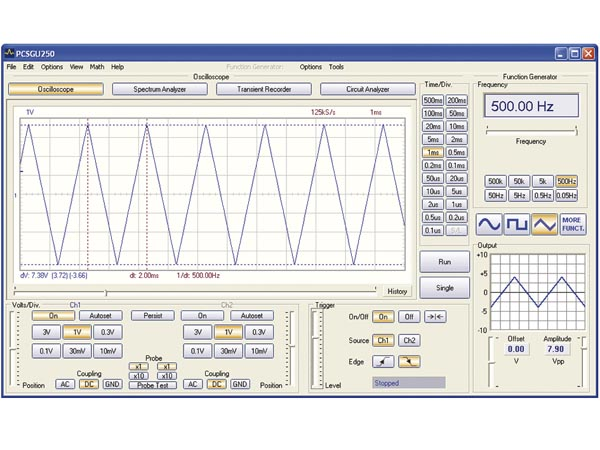
\includegraphics[width=\textwidth]{originalsoft}
\caption{Оригинальное ПО}
\label{originalsoft}
\end{figure}

\begin{figure}[h!]
\centering
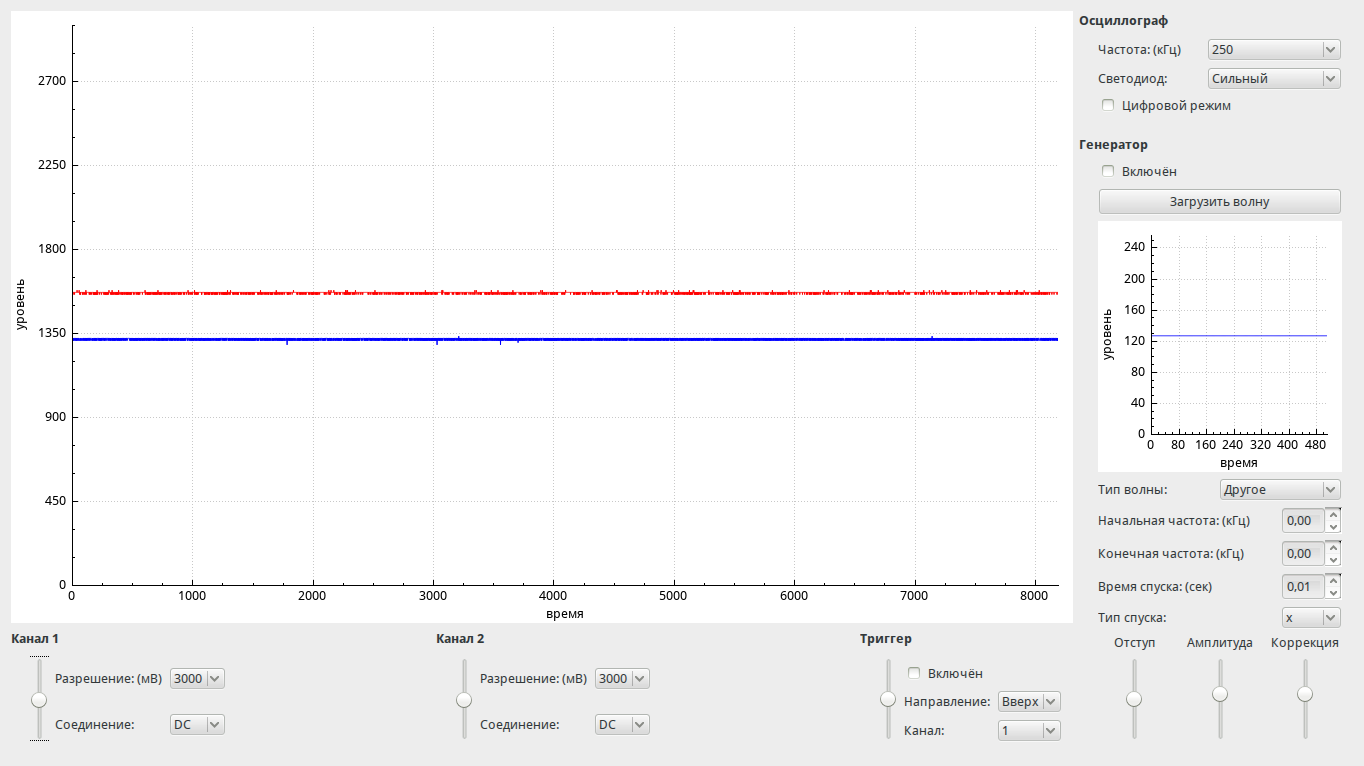
\includegraphics[width=\textwidth]{mysoft}
\caption{Главное окно программы}
\label{mysoft}
\end{figure}

\newpage
\section*{Заключение}
Данный проект был направлен прежде всего на изучение процесса написания модулей,
работающих в режиме ядра, и эта задача была выполнена. Кроме того, был написан
работающий драйвер, поддерживающий почти все изначальные функции осциллографа
(кроме отслеживания внезапных событий), и графический интерфейс пользователя для
него. Было изучено устройство ядра ОС в целом, а также некоторой части её
подсистем, которые были использованы при написании. Также существует
практическая польза от работы, так как такого драйвера ранее не существовало и
он открывает возможности по работе с устройством в ОС GNU/Linux.

\newpage
\printbibliography[heading=bibintoc]

\end{document}